\documentclass[a4paper,11pt]{report}
\usepackage[T1]{fontenc}
\usepackage[utf8]{inputenc}
\usepackage{lmodern,url}
\usepackage{graphicx}
\usepackage{hyperref}
\usepackage{pslatex}
\usepackage{listings}
\usepackage{textcomp}
\usepackage{float}
\usepackage[paper=a4paper,headheight=0pt,left=4cm,top=3cm,right=3cm,bottom=3cm]{geometry}
\usepackage{titling}
\usepackage{pdfpages}
\usepackage{booktabs}
\usepackage[version=4]{mhchem}
\usepackage{isotope}
\usepackage{datetime2}
\usepackage{rotating}
\usepackage{pdflscape}
\usepackage{subfigure}
\DTMsetdatestyle{ddmmyyyy}
\DTMsetup{datesep=--}
\newcommand{\subtitle}[1]{%
  \posttitle{%
    \par\end{center}
    \begin{center}\large#1\end{center}
    \vskip0.5em}%
}
\newcommand{\ra}[1]{\renewcommand{\arraystretch}{#1}}
\newcommand{\addChapter}[1]{\phantomsection \addcontentsline{toc}{chapter}{#1}}
% Tambahkan berkas PDF ke dalam laporan dan gunakan style laporan  
% terhadap berkas ini. 
\newcommand{\inpdf}[1]{
	\includepdf[pages=-,pagecommand={\thispagestyle{fancy}}]{#1.pdf}}
% 
% Tambahkan berkas PDF ke dalam laporan. 
\newcommand{\putpdf}[1]{\includepdf[pages=-]{#1.pdf}}
\renewcommand*\descriptionlabel[1]{\hspace\leftmargin$#1$}
% 
%
% Hyphenation untuk Indonesia 
%
% @author  Andreas Febrian
% @version 1.00
% 
% Tambahkan cara pemenggalan kata-kata yang salah dipenggal secara otomatis 
% oleh LaTeX. Jika kata tersebut dapat dipenggal dengan benar, maka tidak 
% perlu ditambahkan dalam berkas ini. Tanda pemenggalan kata menggunakan 
% tanda '-'; contoh:
% menarik
%   --> pemenggalan: me-na-rik
%

\hyphenation{
    % alphabhet A
    a-na-li-sa a-tur 
    a-pli-ka-si 
    % alphabhet B
    ba-ngun-an 
    be-be-ra-pa 
    ber-ge-rak
    ber-ke-lan-jut-an 
    ber-pe-nga-ruh 
    ber-o-pe-ra-si
    % alphabhet C
    ca-ri cri-ti-cal
    % alphabhet D
    di-sim-pan di-pim-pin de-ngan da-e-rah di-ba-ngun da-pat di-nya-ta-kan 
    di-sim-bol-kan di-pi-lih di-li-hat de-fi-ni-si di-de-fi-ni-si-kan
    di-mo-del-kan di-te-rap-kan
    di-ha-rap-kan
    di-e-va-lu-a-si
    di-su-sun
    di-sa-ji-kan
    % alphabhet E
    e-ner-gi eks-klu-sif
    % alphabhet F
    fa-si-li-tas
    % alphabhet G
    ga-bung-an ge-rak
    % alphabhet H
    ha-lang-an
    % alphabhet I
    % alphabhet J
    % alphabhet K
    ke-hi-lang-an
    ku-ning 
    kua-li-tas ka-me-ra ke-mung-kin-an ke-se-pa-ham-an
    % alphabhet L
    ling-kung-an
    % alphabhet M
    me-ne-ngah
    meng-a-tas-i me-mung-kin-kan me-nge-na-i me-ngi-rim-kan 
    meng-u-bah meng-a-dap-ta-si me-nya-ta-kan mo-di-fi-ka-si
    meng-a-tur
    meng-a-la-mi
    me-re-pre-sen-ta-si-kan
    men-da-pat-kan
    % alphabhet N
    nya-ta non-eks-klu-sif nu-klir
    % alphabhet O
    o-pe-ra-si
    % alphabhet P
	pe-nye-rap-an 
	pe-ngon-trol
    pe-mo-del-an
    pe-ran  pe-ran-an-nya
    pem-ba-ngun-an pre-si-den pe-me-rin-tah prio-ri-tas peng-am-bil-an 
    peng-ga-bung-an pe-nga-was-an pe-ngem-bang-an 
    pe-nga-ruh pa-ra-lel-is-me per-hi-tung-an per-ma-sa-lah-an 
    pen-ca-ri-an peng-struk-tur-an
    per-siap-an pa-ra-me-ter
    pa-sang-an
    % alphabhet Q
    % alphabhet R
    ran-cang-an
    % alphabhet S
    si-mu-la-si sa-ngat
    % alphabhet T
    te-ngah
    ter-da-pat
    % alphabhet U
    % alphabhet V
    % alphabhet W
    % alphabhet X
    % alphabhet Y
    % alphabhet Z
    % special
}


\renewcommand{\contentsname}{Daftar Isi}
\renewcommand{\chaptername}{BAB}
\renewcommand{\bibname}{Daftar Referensi}
\renewcommand{\listfigurename}{Daftar Gambar}
\renewcommand\lstlistlistingname{Daftar Program}
\renewcommand{\figurename}{Gambar}
\renewcommand{\tablename}{Tabel}
%\title{Lampiran II}
%\title{Kajian Komputasi Dinamika Fluida berbasis OpenFOAM}
%\author{Arya Adhyaksa Waskita}
%\date{January 31, 2017}
\begin{document}
\begin{titlepage}

\newcommand{\HRule}{\rule{\linewidth}{0.5mm}} % Defines a new command for the horizontal lines, change thickness here

\center % Center everything on the page


%----------------------------------------------------------------------------------------
%	LOGO SECTION
%----------------------------------------------------------------------------------------


\includegraphics[scale=.25]{pics/logo.png}\\[1cm] % Include a department/university logo - this will require the graphicx package

%----------------------------------------------------------------------------------------
%	TITLE SECTION
%----------------------------------------------------------------------------------------

\HRule \\[0.4cm]
{ \huge \bfseries Dokumen Pengembangan TRIAC \\ (TRIso \textit{Analysis Code})}\\[0.4cm] % Title of your document
\HRule \\[1.5cm]

%----------------------------------------------------------------------------------------
%	HEADING SECTIONS
%----------------------------------------------------------------------------------------
%\textsc{Sub Bidang Termohidrolika}\\[0.25cm] % Minor heading such as course title
\textsc{Laboratorium Komputasi}\\[0.25cm] % Major heading such as course name
\textsc{\Large Pusat Teknologi dan Keselamatan Reaktor Nuklir}\\[1.5cm] % Name of your university/college

 
%----------------------------------------------------------------------------------------
%	AUTHOR SECTION
%----------------------------------------------------------------------------------------

\begin{minipage}{0.4\textwidth}
\begin{flushleft} \large
\emph{Disusun oleh:}\\
Arya Adhyaksa Waskita
\end{flushleft}
\end{minipage}
~
\begin{minipage}{0.4\textwidth}
\begin{flushright} \large
\emph{Supervisor:} \\
Dr. Eng. Topan Setiadipura
\end{flushright}
\end{minipage}\\[4cm]

% If you don't want a supervisor, uncomment the two lines below and remove the section above
%\Large \emph{Author:}\\
%John \textsc{Smith}\\[3cm] % Your name

%----------------------------------------------------------------------------------------
%	DATE SECTION
%----------------------------------------------------------------------------------------

{\large \today}\\[3cm] % Date, change the \today to a set date if you want to be precise
%{\large 31 Juli 2017}\\[3cm] % Date, change the \today to a set date if you want to be precise
 
%----------------------------------------------------------------------------------------

\vfill % Fill the rest of the page with whitespace

\end{titlepage}

%\tableofcontents

\pagenumbering{roman}
%\maketitle
\clearpage
\setcounter{page}{2}
\addChapter{Daftar Gambar}
\tableofcontents
%\clearpage
\listoffigures
\addChapter{Daftar Program}
\lstlistoflistings
%\clearpage
\pagenumbering{arabic}

\chapter{Pendahuluan}
BATAN saat ini tengah berencana membangun reaktor riset baru berbasis HTGR (\textit{High Temperature Gas-cooled Reactor}) \cite{wang2004integrated} sebagai persiapan PLTN, yang akan dibangun di Indonesia di masa depan \cite{rde}. Salah satu yang perlu diperhatikan dalam pengembangan reaktor jenis ini adalah bahan bakarnya yang berjenis \textit{pebble} yang bentuknya dapat diilustrasikan seperti pada Gambar \ref{fig:bentukpebble}. Bahan bakar harus dirancang sedemikian rupa sehingga rasio gagalnya bahan bakar selama operasi minimal. 

\begin{figure}[h]
  \centering
  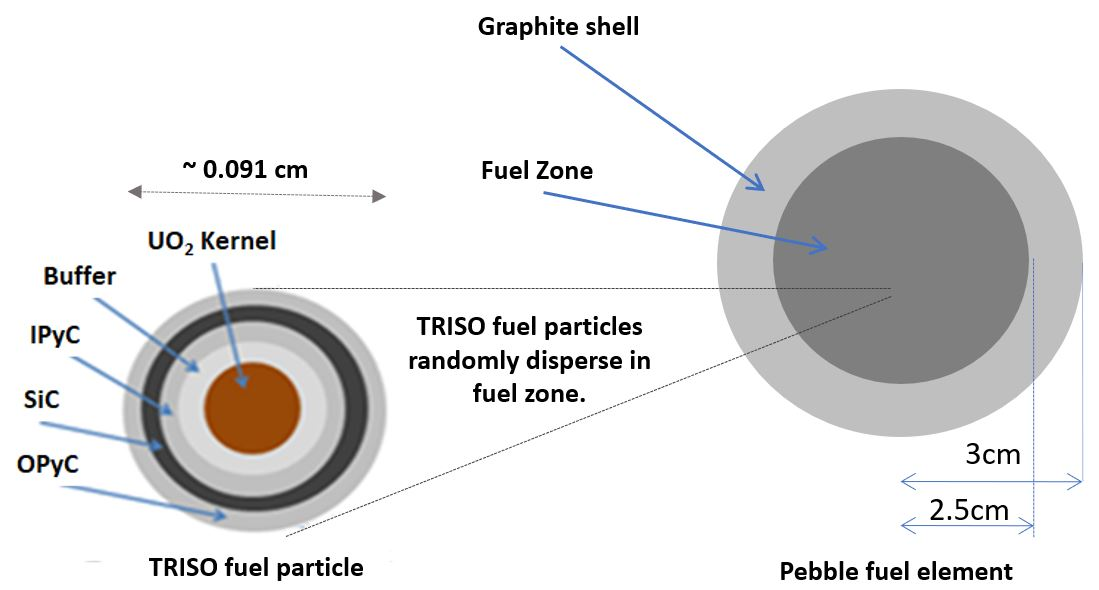
\includegraphics[scale=.5]{pics/triso.JPG}
  \caption[Ilustrasi bentuk bahan bakar \textit{pebble}]{Ilustrasi bentuk bahan bakar \textit{pebble} \cite{tsdipura}}
  \label{fig:bentukpebble}
\end{figure} 

Bahan bakar berjenis \textit{pebble} ini memiliki komponen utama yang dalam Gambar \ref{fig:bentukpebble} disebut sebagai \textit{triso fuel particle}, dengan triso adalah \textit{tri structural isotrophic}. Dalam upaya menguasai teknologi reaktor berjenis HTGR melalui pengembangan RDE, salah tugas yang harus dilaksanakan adalah penguasaan analisis kegagalan bahan bakarnya, khususnya ketika terjadi kecelakaan.

Beragam model analisis telah dikembangkan, salah satunya yang dikembangkan oleh Wang \cite{wang2004integrated}. Selain itu, terdapat sebuah model sederhana yang dikembangkan oleh Verfondern dalam PANAMA \cite{VERFONDERN201484}. Pada model tersebut, bahan bakar disebut gagal jika kekuatan lapisan SiC (\textit{Silicon Carbide}) lebih kecil daripada tekanan internal dari lapisan di bawahnya. Model inilah yang akan diterapkan dalam TRIAC (\textit{TRIso Analysis Code}).

\chapter{Alur Perhitungan}
\section{Pendahuluan}
Secara umum, perhitungan TRIAC mengikuti diagram alir seperti pada Gambar \ref{fig:flowchart} berikut. Penerapannya disajikan dalam Listing \ref{triac.py} berdasarkan pengetahuan yang diperoleh dari dokumen teknis PANAMA \cite{report1}. Meski diagram alir tersebut tergambar secara sekuensial, tetapi secara perhitungan ada beberapa formula yang tidak saling tergantung, sehingga urutannya dapat saja dibalik. Hubungan saling ketergantungan antar formula disajikan dalam Gambar \ref{fig:irradiasi} dan \ref{fig:accident}. 
\begin{figure}[h]
  \centering
  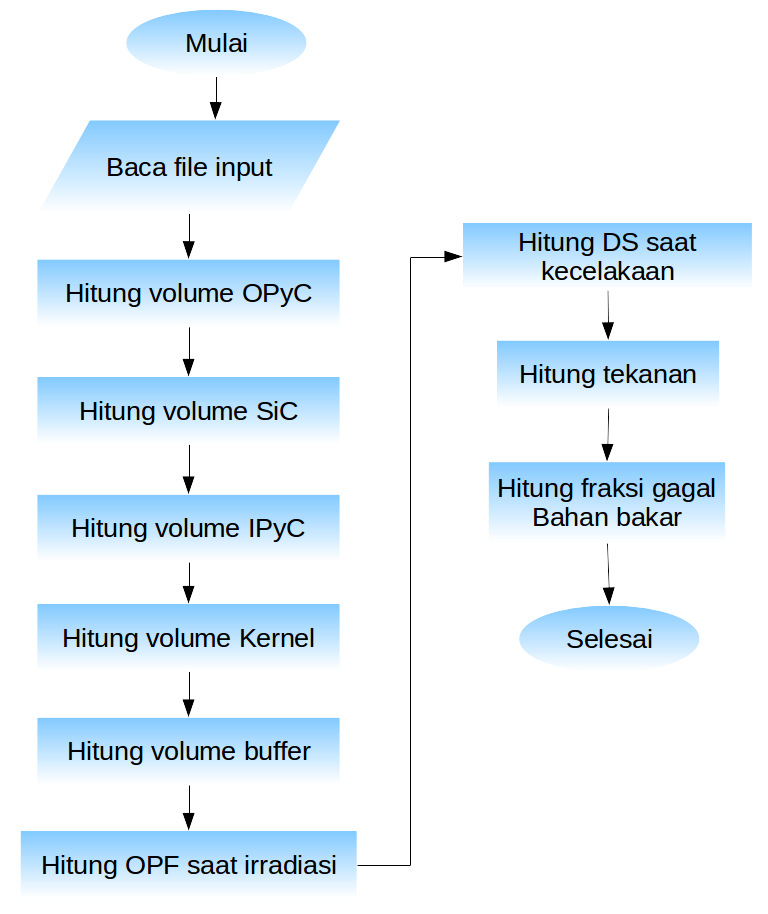
\includegraphics[scale=.5]{pics/Flowchart.png}
  \caption{Diagram alir perhitungan TRIAC}
  \label{fig:flowchart}
\end{figure}

\section{Membaca \textit{file input}}
Sub rutin ini ditujukan untuk membaca \textit{file input} dengan format seperti terdapat pada Lampiran \ref{lamp:inputExample}. Sub rutin ini menggunakan skema yang kaku karena identifikasi nilai-nilai yang akan dibaca ditentukan oleh suatu teks tertentu. Setelah teks yang menjadi penanda, nilai-nilai yang dibutuhkan dibaca. Tetapi, nilai tersebut dapat langsung berada dalam satu baris bersama dengan teks penanda, atau berada pada baris yang berbeda. Sub rutin ini terdapat pada Listing \ref{InputData.py} dan akan dijelaskan pada sub bab \ref{sec:introPenerapan}.
 
\section{Menghitung OPF saat irradiasi}
\label{sec:OPF}
OPF (\textit{Oxygen Per Fission}) adalah jumlah atom oksigen yang terlepas selama fisi atom $U^{235}$ atau $Pu^{239}$. Atom oksigen ini mempengaruhi terbentuknya senyawa CO yang akan meningkatkan tekanan internal dalam bahan bakar. Pembentukan senyawa CO juga dipengaruhi oleh temperatur, waktu serta jenis partikel kernel. 

Nilai OPF didekati oleh persamaan (\ref{eq:opf1}). Nilai $n$ dalam persamaan (\ref{eq:opf1}) sama dengan banyaknya data sejarah irradiasi. Nilai $\Delta_{i}$ merupakan selisih waktu dari sejarah irradiasi yang dicatat. Nilainya akan berubah dengan berubahnya rentang pencatatan temperatur irradiasi. Jika dalam contoh kasus yang disajikan pada Lampiran 1, rentang waktu pencatatan temperatur irradiasi dilakukan setiap $17$ hari, maka $\Delta_{i}$ adalah $17$ hari atau $17 x 24 x 3600$ detik. $t_B$ adalah waktu irradiasi total bahan bakar, sedangkan $\overline{t_i}$ waktu irradiasi ketika pencatatan dilakukan.

\begin{equation}
  OPF \simeq \sum_{i=1}^{n} g(\overline{t_{i}}) \cdot (t_{B}-\overline{t_{i}}) \cdot \Delta t_{i}
  \label{eq:opf1}
\end{equation}
 
Tetapi, nilai OPF juga didefinisikan seperti persamaan (\ref{eq:opf2}), dengan nilai $g(\overline{t_{i}})$ didefinisikan oleh persamaan (\ref{eq:gt}). Nilai $R$ pada persamaan (\ref{eq:gt}) adalah konstanta gas sebesar $8.3143 [\frac{J}{mole \cdot K}]$.
\begin{equation}
  OPF = \frac{g(T)}{2} \cdot t^2
  \label{eq:opf2}
\end{equation} 
 
\begin{equation}
  \frac{g(T)}{2}=8.32 \cdot 10^{-11} \cdot e^{\frac{-163000}{R \cdot T}}
  \label{eq:gt}
\end{equation} 
 
Nilai OPF selanjutnya digunakan untuk menghitung nilai temperatur irradiasi ($T_B$) dari persamaan (\ref{eq:TB}). Formula empiris tersebut sesuai untuk jenis bahan bakar $UO_2$.
\begin{equation}
  \log OPF=-10.08-\frac{0.85 \cdot 10^4}{T_B} + 2 \cdot \log t_B
  \label{eq:TB}
\end{equation} 

Sedangkan nilai $T_B$ akan digunakan untuk menghitung $DS$, faktor berkurangnya koefisien difusi ($s^{-1}$) dari gas hasil fisi di dalam partikel kernel. Nilainya untuk bahan bakar $UO_2$ memenuhi persamaan (\ref{eq:DS}).

\begin{equation}
  \log DS=-2.30-\frac{0.8116 \cdot 10^4}{T_B}
  \label{eq:DS}.
\end{equation}

Terakhir, $DS$ akan digunakan untuk menghitung sebuah nilai tak berdimensi $\tau_i$ yang memenuhi persamaan (\ref{eq:taui}).
\begin{equation}
  \tau_i=DS(T_B) \cdot t_B
  \label{eq:taui}
\end{equation}

\section{Menghitung DS saat kecelakaan}
Seperti telah dijelaskan dalam sub bab \ref{sec:OPF}, $DS$ adalah faktor berkurangnya koefisien difusi gas hasil fisi dalam partikel kernel. Sekarang, faktor ini dihitung ketika kondisi kecelakaan terjadi. Kita memerlukan sejarah temperatur bahan bakar setelah kecelakaan terjadi serta $\tau_i$. yang telah dihitung di persamaan (\ref{eq:taui}).

Dengan menggunakan persamaan (\ref{eq:taui}), kita dapat menghitung nilai $DS$ dengan temperatur kecelakaan yang tercatat.  Kemudian, kita perlu menghitung nilai $\tau_A$ dengan persamaan (\ref{eq:taui}) tetapi dengan nilai temperatur dan waktu setelah terjadi kecelakaan. Selanjutnya, dengan modal nilai $\tau_i$ dan $\tau_A$ kita akan menghitung nilai $Fd$, yang merupakan faktor fisi gas Xe dan Kr (yang dominan). Nilai $Fd$ dihitung dengan persamaan (\ref{eq:Fd}).
\begin{equation}
  Fd=\frac{(\tau_i + \tau_A) \cdot f(\tau_i + \tau_A) - \tau_A \cdot f(\tau_A)}{\tau_i}
  \label{eq:Fd}
\end{equation}

Sedangkan nilai $f(\tau)$ dihitung menggunakan persaamaan (\ref{eq:ftau}). Batas atas nilai $n$ pada persaamaan (\ref{eq:ftau}) dapat menggunakan nilai yang cukup besar, misalnya $1000$, atau ketika dua nilai berdekatan yang dihasilkan hanya berselisih kurang dari $10^{-20}$. Idealnya, suku penjumlahan sebanyak $n$ akan semakin baik jika hasilnya mendekati $1$.
\begin{equation}
  f(\tau)=1-\frac{6}{\tau} \cdot \sum_{n=1}^{\infty} \left( \frac{1-e^{-n^2 \cdot \pi^2 \cdot \tau}}{n^4 \cdot \pi^4} \right)
  \label{eq:ftau}
\end{equation}

%Di level implementasi, perhitungan $DS$ saat kecelakaan didistribusi ke dalam beberapa fungsi seperti terlihat pada Listing \ref{triac.py}. Masing-masing fungsi tersebut adalah \texttt{DS(accident,tauI)} dan \texttt{FD(tauA,tauI)}.

\section{Menghitung tekanan}
Tekanan adalah variabel yang penting dalam tahapan analisis ini karena akan menentukan fraksi gagal bahan bakar. PANAMA \cite{report1} memodelkan fraksi gagal partikel bahan bakar dari sejauh mana lapisan silikon karbida mampu menahan tekanan akibat rilisnya gas produk fisi. Untuk menghitung tekanan yang timbul ketika kecelakaan terjadi pada waktu tertentu, sehingga menyebabkan panas tertentu, digunakan persamaan (\ref{eq:tekanan}) \cite{report1}. 
\begin{equation}
  p=\frac{(F_d \cdot F_f + OPF) \cdot F_b \cdot (\frac{V_k}{V_m}) \cdot R \cdot T}{ V_f}
  \label{eq:tekanan}
\end{equation}
dengan :
\begin{description}
  \item $F_d$ = fraksi relatif gas fisi yang lepas 
  \item $F_f$ = produk fisi yang dihasilkan dari gas fisi stabil, $F_f$=0.31
  \item OPF = jumlah atom oksigen setiap terjadi fisi saat terjadi kecelakaan
  \item $F_b$ = \textit{burnup} logam berat (FIMA)
  \item $V_f$ = fraksi void [$m^3$], terkait dengan $50\%$ volume buffer 
  \item $V_k$ = volume kernel [$m^3$]
  \item $V_m$ = volume molar dalam partikel kernel $\left[\frac{m^3}{mole} \right]$, didefinisikan sebagai rasio berat 1 mol material kernel terhadap kerapatannya. Menurut Verfondern \cite{report1}, $V_m$ untuk $(Th,U)O_2$, $UO_2$ dan UCO masing-masing adalah $2.52 \cdot 10^{-5}[\frac{m^3}{mole}]$, $2.44 \cdot 10^{-5}[\frac{m^3}{mole}]$ dan $2.51 \cdot 10^{-5}[\frac{m^3}{mole}]$.
  \item $R$ = konstanta gas, 8.3143 $\left[\frac{J}{(mole \cdot K)} \right]$
\end{description}

Khusus untuk variabel $OPF$, karena perhitungan tekanan dilakukan ketika terjadi kecelakaan, digunakanlah persamaan (\ref{eq:opf3}). Persamaan (\ref{eq:opf3}) mirip dengan persamaan (\ref{eq:TB}) dengan penambahan suku ke-3.
\begin{equation}
  \log OPF=-10.08-\frac{0.85 \cdot 10^4}{T_B} + 2 \cdot \log t_B - 0.04 \cdot \left( \frac{10^4}{T} + \frac{10^4}{T_B + 75} \right)
  \label{eq:opf3}
\end{equation}

\section{Fraksi gagal bahan bakar}
Tahapan terkahir dari analisis ini adalah perhitungan fraksi gagal bahan bakar. Secara umum, fraksi gagal bahan bakar dipengaruhi sejumlah sebab. Dalam analisis yang dilakukan TRIAC (dan juga PANAMA sebagai acuannya), gagalnya bahan bakar dapat disebabkan oleh 3 sebab. Ketiganya adalah sebagai berikut.
\begin{enumerate}
\item Pabrikasi ($\phi_0$). Dalam analisis ini, nilai $\phi_0$ diasumsikan sama dengan $0$.
\item Berkurangnya \textit{tensile strength} lapisan SiC ($\phi_1$). Hal ini dapat terjadi karena
\begin{itemize}
\item proses irradiasi maupun
\item meningkatnya temperatur secara signifikan ketika terjadi kecelakaan) atau disebut juga \textit{grain boundary}.
\end{itemize}  
\item Dekomposisi termal pada temperatur tinggi yang menyebabkan terjadinya \textit{weight loss} pada lapisan SiC ($\phi_2$).
\end{enumerate}

Ketiga sebab terjadinya kegagalan bahan bakar tersebut mengikuti persamaan (\ref{eq:gagal1}).
\begin{equation}
  \phi_{total}=1-(1-\phi_0) \cdot(1-\phi_1) \cdot (1-\phi_2)
  \label{eq:gagal1}
\end{equation}

\subsection{Fraksi gagal akibat berkurangnya \textit{tensile strength}}
Fraksi gagal partikel triso dimodelkan dengan apa yang diistilahkan Verfondern sebagai model bejana tekan \cite{report1}. Hal ini disebabkan karena  fraksi gagal dipengaruhi oleh variabel-variabel yang terenkapsulasi dalam parameter tenanan internal dan kekuatan lapisan silikon karbida. Nilai fraksi gagal bahan bakar pada waktu $t$ setelah terjadinya kecelakaan diperoleh dengan persamaan (\ref{eq:gagal}).
\begin{equation}
  \phi_1(t,T)=1-e^{-\ln 2 \cdot \left(\frac{\sigma_t}{\sigma_o}\right)^m}
  \label{eq:gagal}
\end{equation}
dengan :
\begin{description}
  \item $\sigma_o$=\textit{tensile strength} dari SiC [Pa] pada akhir irradiasi
  \item $\sigma_t$=tekanan yang dialami SiC [Pa] akibat tekanan gas internal
  \item $m$=parameter Weibull (dijelaskan selanjutnya)
\end{description}

Variabel tekanan internal pada SiC ($\sigma_t$) dihitung dengan dengan persamaan (\ref{eq:sigmaT}). Pada persamaan (\ref{eq:sigmaT}), jari-jari lapisan SiC merupakan rerata karena lapisan SiC memang memiliki ketebalan yang nilai awalnya diwakili oleh variabel $d_o$.
\begin{equation}
  \sigma_t =\frac{r \cdot p}{2 \cdot d_o} \cdot \left( 1+\frac{\dot{v} \cdot t}{d_o} \right)
  \label{eq:sigmaT}
\end{equation}
dengan :
\begin{description}
  \item $r$=rerata jari-jari SiC, $\left( 0.5 \cdot \left( r_a^3 + r_i^3 \right)\right)^{\frac{1}{3}}$ [m]
  \item $d_o$=ketebalan awal lapisan SiC, $r_a - r_i$ [m]
  \item $p$=tekanan gas fisi dalam partikel [Pa], dihitung menggunakan persamaan (\ref{eq:tekanan})
  \item $\dot{v}$=laju korosi sebagai fungsi temperatur (T), $\left[\frac{m}{s}\right]$
\end{description}

Sedangkan variabel laju korosi ($\dot{v}$) dihitung dengan persamaan (\ref{eq:korosi}), mirip dengan persamaan (\ref{eq:gt}) dengan perbedaan pada konstanta.
\begin{equation}
  \dot{v}=5.87 \cdot 10^{-7} \cdot e^{-\left( \frac{179500}{R \cdot T}\right)}
  \label{eq:korosi}
\end{equation}

Selanjutnya, variabel \textit{tensile strength} lapisan SiC, penurunan nilainya mengikuti persamaan (\ref{eq:strengthSiC}). Variabel $\sigma_{oo}$ merupakan \textit{tensile strength} awal sebelum diiradiasi. Nilainya merupakan sesuatu yang dapat diukur. Sedangkan $\Gamma$ dan $\Gamma_s$ masing-masing merupakan \textit{fluence} netron cepat $\left[ 10^{25}m^{-2} EDN\right]$ dan \textit{fluence} yang dipengaruhi temperatur irradiasi. Nilai $\Gamma_s$ ditentukan menggunakan persamaan (\ref{eq:fluenceS}). %Nilai minimum $\sigma_{oo}$ merupakan nilai awal \textit{tensile strength} dan diasumsikan sama dengan 196 [MPa]. Tentunya, dengan perlakuan irradiasi yang sama, lapisan SiC dengan nilai awal \textit{tensile strength} terkecil akan memiliki nilai akhir \textit{tensile strength} yang juga kecil.
\begin{equation}
  \sigma_o = \sigma_{oo} \cdot \left( 1- \frac{\Gamma}{\Gamma_s} \right)
  \label{eq:strengthSiC}
\end{equation}

\begin{equation}
  \log \Gamma_s = 0.556 + \frac{0.065 \cdot 10^4}{T_B}
  \label{eq:fluenceS}
\end{equation}

\textit{Tensile strength} lapisan SiC yang dihitung menggunakan persamaan (\ref{eq:strengthSiC}) merupakan nilai yang berlaku pada satu \textit{coated particle}. Padahal, ada sangat banyak \textit{coated particle} yang dioperasikan. Karena itu, diperlukan perhitungan yang mempertimbangkan variabel ini untuk semua distribusi \textit{coated particles}. Dengan pendekatan yang sama seperti persamaan (\ref{eq:strengthSiC}), persamaan (\ref{eq:strengthSiCdist}) dibangun. Nilai $\Gamma_m$ ditentukan menggunakan persamaan (\ref{eq:fluenceM}).

\begin{equation}
  m_o = m_{oo} \cdot \left( 1- \frac{\Gamma}{\Gamma_m} \right)
  \label{eq:strengthSiCdist}
\end{equation}

\begin{equation}
\log \Gamma_m = 0.394 + \frac{0.065 \cdot 10^4}{T_B}
\label{eq:fluenceM}
\end{equation}

%Nilai $m_o$ pada persamaan (\ref{eq:strengthSiCdist}) kemudian akan disubstitusi ke persamaan (\ref{eq:gagal}) sebagai $m$. Pada konteks ini, parameter $m$ yang merupakan salah satu parameter dalam persamaan (\ref{eq:gagal}) ditentukan berdasarkan kekuatan (\textit{tensile strength}) lapisan SiC. $m$ menentukan distribusi kekuatan SiC pada sejumlah partikel TRISO. 

Sama seperti $\sigma_{oo}$, nilai $m_{oo}$ juga diperoleh dengan mengukur parameter tersebut pada partikel yang belum diiradiasi. Tabel \ref{tab:oo} menunjukkan nilai $\sigma_{oo}$ dan $m_{oo}$ pada beberapa jenis specimen sebelum dikenakan irradiasi \cite{report1}.%Nilainya akan berkurang sejalan dengan proses irradiasi serta mengikuti persamaan (\ref{eq:gagal}). 


\begin{table}
  \caption[Nilai $\sigma_{oo}$ dan $m_{oo}$ untuk berbagai jenis specimen]{Nilai $\sigma_{oo}$ dan $m_{oo}$ untuk berbagai jenis specimen\cite{report1}}
  \label{tab:oo}

  \begin{center}
  \ra{1.3}
    \begin{tabular}{@{}lrrcrr@{}}\toprule
    %\hline
    Specimen & \multicolumn{2}{c}{Sebelum irradiasi} & \phantom{abc} & \multicolumn{2}{c}{Setelah irradiasi} \\ \cmidrule{2-3} \cmidrule{5-6} 
       & $\sigma_{oo}$ [MPa] & $m_{oo}$ && $\sigma_{o}$ [MPa] & $m_{o}$ \\ \midrule%\hline
       EO 1674 & 722 & 7.0 && 660 & 6.1\\
       EO 1607 & 850 & 8.0 && 777 & 7.0\\
       HT 150-167 & 600 & 6.0 && 549 & 5.3\\
       EO 249-251 & 453 & 5.0 && 414 & 4.4\\
       EO 403-405 & 867 & 8.4 && 793 & 7.4\\
       EUO 1551 & 1060 & 8.5 && 969 & 7.4\\
       ECO 1541 & 1080 & 6.4 && 987 & 5.6\\
       EC 1338 & 998 & 7.4 && 912 & 6.5\\ %\hline 
       \bottomrule
    \end{tabular}
  \end{center}
\end{table}


Selain korosi karena proses irradiasi, lapisan SiC juga dapat terkorosi karena \textit{grain Boundary}. Jika korosi akibat irradiasi tergantung pada sejarah irradiasi yang dialami bahan bakar dan terjadi sebelum kecelakaan, maka korosi karena \textit{grain Boundary} terjadi setelah kecelakaan. Penurunan nilai distribusi \textit{tensile strength} akibat meningkatnya temperatur karena kecelakaan mengikuti persamaan (\ref{eq:grainBoundary}), di mana nilai $m_o$ diperoleh dari persamaan (\ref{eq:strengthSiCdist})
\begin{equation}
  m=m_o \cdot \left( 0.44 + 0.56 \cdot e^{-\dot{\eta} \cdot t}\right)
  \label{eq:grainBoundary}
\end{equation}

dan nilai $\dot{\eta}$ mengikuti persamaan {\ref{eq:eta}} dengan pola yang sama seperti persamaan (\ref{eq:korosi}).
\begin{equation}
  \dot{\eta}=0.565 \cdot e^{\left(\frac{-187400}{R \cdot T}\right)} [s^{-1}]
  \label{eq:eta}
\end{equation}

\subsection{Fraksi gagal bahan bakar akibat \textit{weight loss}}
Laju \textit{weight loss} yang terjadi akibat tingginya temperatur saat terjadi kecelakaan mengikuti persamaan (\ref{eq:weightLoss}).
\begin{equation}
  k=k_o \cdot e^{\frac{-Q}{R \cdot T}}
  \label{eq:weightLoss}
\end{equation}
dengan $Q=556 \left[ \frac{kJ}{mol}\right]$ dan $k_o$ adalah faktor frekuensi yang tergantung pada jenis partikel.

Selanjutnya, diasumsikan bahwa partikel TRISO tergantung pada apa yang disebut sebagai ''\textit{action integral}'', dan disimbolkan dengan $\zeta$ yang nilainya mengikuti persamaan (\ref{eq:zeta}).
\begin{equation}
  \zeta=\int_{t_1}^{t_2} k(T) dt
  \label{eq:zeta}
\end{equation}
dengan $K(T)$ adalah nilai yang menggambarkan sejarah kondisi partikel yang bergantung pada temperatur dan waktu.

Secara numerik, persamaan (\ref{eq:zeta}) dapat dituliskan sebagai persamaa (\ref{eq:zeta1}).
\begin{equation}
  \zeta(t_2)=\zeta(t_1)+k(T_m) \cdot (t_2 - t_1)
  \label{eq:zeta1}
\end{equation}
dengan $k(T_m)=\frac{375}{d_o} \cdot e^{\left(\frac{-556000}{R \cdot T_m}\right)}$.

Kemudian, fraksi gagal $\phi_2$ sedemikian rupa sehingga nilainya $\leq 1$. Karena itu, variabel $\phi_2$ selanjutnya didefinisikan sebagai persamaan (\ref{eq:phi2}).
\begin{equation}
\phi_2(t,T)=1-e^{-\alpha \cdot \zeta^{\beta}}
\label{eq:phi2}
\end{equation}

Nilai $\alpha$ dan $\beta$ kemudian ditentukan secara empiris. Dan berdasarkan penelitian empiris sebelumnya terhadap partikel $UO_2$, diperoleh nilai $\alpha=\ln 2=0.693$, sedangkan nilai $\beta=0.88$.

Dalam TRIAC, faktor fraksi gagal ini tidak akan dipertimbangkan. Hal ini disebabkan karena kondisi ini terjadi pada temperatur di atas $2000\,^{\circ}{\rm C}$. Sementara RDE tidak dirancang untuk sampai pada temperatur tersebut.

\subsection{Pertumbuhan fraksi gagal}
Berdasarkan PANAMA \cite{report1}, Verfondern memodelkan pertumbuhan fraksi gagal partikel triso akibat berkurangnya \textit{tensile strength} adalah seperti persamaan (\ref{eq:fraksigagal}) berikut.
\begin{equation}
\phi_1=\phi_1(t_2,T_m)-\phi_1(t_1,T_m)
\label{eq:fraksigagal}
\end{equation}

$T_m$ merupakan temperatur rata-rata antara waktu $t_1$ dan $t_2$. Ilustrasinya disajikan dalam Gambar \ref{fig:pertumbuhanPhi} 
\begin{figure}
  \begin{center}
    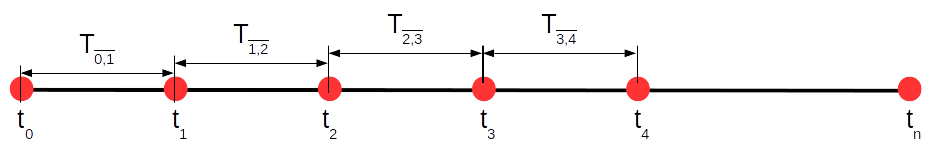
\includegraphics[scale=.5]{pics/akumulasiPhi.png}
    \caption{Hubungan antara waktu dan temperatur pada perhitungan $\phi_1$}
    \label{fig:pertumbuhanPhi}
  \end{center}
\end{figure}

Disebutkan Verfondern \cite{report1}, nilai $\phi_1$ saat kecelakaan dimulai ($t_0$ seperti pada Gambar \ref{fig:pertumbuhanPhi}) merupakan fungsi dari sejarah irradiasi. Sedangkan untuk waktu-waktu selanjutnya ($t_1, t_2, \cdots, t_n$) merupakan akumulasi dari nilai $\phi_1$ pada persamaan (\ref{eq:fraksigagal}). Jika $\phi_1$ pada $t_1$ lebih besar daripada $\phi_1$ pada saat $t_0$, maka akumulasikan nilai $\phi_1$. Jika sebaliknya, gunakan nilai $\phi_1$ sebelumnya untuk perhitungan selanjutnya (nilai $\phi_1$ tetap). 

Sebagai ilustrasi, saat menghitung nilai $\phi_1$ di $t=t_1$, maka diperlukan nilai $\phi_1(t_0, T_m)$ (nilai pertama) dan $\phi_1(t_1, T_m)$ (nilai kedua). Nilai pertama adalah fungsi irradiasi, sedangkan nilai kedua diperoleh dari persamaan (\ref{eq:gagal}) dengan parameter-parameter yang sesuai. Selisih keduanya akan menentukan nilai $\phi_1$ di titik $t=t_1$. Jika selisih nilai kedua dan pertama positif, selisih nilai tersebut diakumulasikan pada nilai $\phi_1$ di $t=t_0$. Tetapi jika sebaliknya, maka nilai $\phi_1$ di titik $t=t_1$ sama dengan nilai $\phi_1$ di titik $t=t_0$. Skenario yang sama berlaku untuk titik-titik waktu selanjutnya.

\section{Modul \textit{sampling}}
\label{sec:lhs}
\subsection{Pendahuluan}
\textit{Latin Hypercube Sampling} (LHS) saat ini telah menjadi metode sampling yang paling banyak digunakan dalam analisis keandalan dan ketidakpastian pada analisis sistem kompleks berbasis Monte-Carlo \cite{HELTON200323,SHIELDS201696}. LHS sendiri didefinisikan sebagai metode untuk menghasilkan \textit{sample} acak dari nilai parameter \cite{lhs}. Alasan LHS banyak digunakan dalam metode berbasis Monte Carlo adalah karena kemampuannya mengurangi jumlah eksekusi untuk memperoleh hasil yang cukup akurat.

LHS dapat dimodelkan sebagai sebuah fungsi $y=f(x)$, dengan $f$ merepresentasikan model dari sistem yang sedang dikaji, $x=[x_1, x_2, \ldots]$ merupakan vektor input bagi model, dan $y=[y_1, y_2, \ldots]$ merupakan vektor prediksi model \cite{HELTON200323}. Tujuan dari analisis ketidakpastian ini adalah untuk menentukan ketidakpastian elemen $y$ sebagai akibat dari ketidakpastian elemen $x$. Dalam konteks TRIAC, LHS dapat digunakan untuk menentukan ketidakpastian fraksi gagal bahan bakar triso sebagai akibat ketidakpastian dimensi partikel tersebut. Tabel \ref{tab:variasi} menunjukkan contoh ketidakpastian parameter dalam partikel triso \cite{report2}

TRIAC selanjutnya juga akan dilengkapi dengan SRS (Simple Random Sampling). LHS dan SRS selanjutnya digabung menjadi modul \textit{sampling} pada TRIAC.

\begin{table}[h!] % <--
  \begin{center}
\caption[Nilai nominal dan variasinya pada komposisi partikel triso]{Nilai nominal dan variasinya pada komposisi partikel triso\cite{report2}}  
\label{tab:variasi}
\scriptsize
\ra{1.3}
  \begin{tabular}{p{4.5cm}p{1.8cm}p{2cm}p{2.6cm}p{2cm}p{2cm}} \toprule
Item & Nilai Nominal & Toleransi disain & Rentang teramati & Standar deviasi \\ \midrule
Uranium fuel loading ($\frac{g}{fuel\;pebble}$) & $5.0g$ & $5.0\;\pm\;0.1g$ & $4.95-5.05g$ & n/a \\
Density of graphite in matrix and outer shell of fuel pebble & $1.73\frac{g}{cm^3}$ & $1.75\;\pm\;0.02\frac{g}{cm^3}$ & $1.73\frac{g}{cm^3}$ & n/a \\
Total ash in fuel element & $0$ & $\leq\;300.0\;ppm$ & $130-190\;ppm$ & n/a \\
Lithium in fuel element & $0$ & $\leq\;0.3\;ppm$ & $0.007-0.023\;ppm$ & n/a \\
Boron in fuel element & 1.3\;ppm & $\leq\;0.3\;ppm$ & $0.15\;ppm$ & n/a \\
Ratio of oxygen to uranium in kernel & 2 & $<2.01$ & n/a & n/a \\
Density of kernel & $10.4\frac{g}{cm^3}$ & $>10.4\frac{g}{cm^3}$ & $10.83\frac{g}{cm^3}$ & n/a \\
Density of buffer layer & $1.1\frac{g}{cm^3}$ & $\leq\;1.1\frac{g}{cm^3}$ & $1.02\frac{g}{cm^3}$ & teramati $0.03\frac{g}{cm^3}$\\
Density of IPyC layer & $1.9\frac{g}{cm^3}$ & $1.1\;\pm\;0.1\frac{g}{cm^3}$ & $1.86\;\pm\;0.06\frac{g}{cm^3}$ & n/a \\
Density of SiC layer & $3.18\frac{g}{cm^3}$ & $\geq\;3.18\frac{g}{cm^3}$ & $3.21\;\pm\;0.02\frac{g}{cm^3}$ & n/a \\
Density of OPyC layer & $1.9\frac{g}{cm^3}$ & $1.9\;\pm\;0.1\frac{g}{cm^3}$ & $1.87\;\pm\;0.02\frac{g}{cm^3}$ & n/a \\
Density of reflector graphite & $1.6\frac{g}{cm^3}$ & n/a & n/a & n/a \\
\bottomrule
\end{tabular}
\end{center}
\end{table}
\normalsize

\subsection{Opsi distribusi}
LHS bekerja dengan tahapan sebagai berikut \cite{mbasinta}.
\begin{enumerate}
  \item Mendefinisikan variabel $Y=f(x_i)$. Pendefinisian variabel $Y$ melibatkan
  \begin{itemize}
    \item jumlah variabel $X$
    \item konstanta setiap variabel $x_i$
  \end{itemize}
  \item Mendefinisikan variabel $X$. Beberapa tahapan yang perlu dilakukan adalah sebagai berikut.
  \begin{itemize}
    \item Menentukan jenis distribusi. Untuk TRIAC, jenis distribusi yang akan digunakan adalah normal, \textit{uniform} dan triangular. Sample yang dihasilkan jumlahnya akan mengikuti distribusi yang ditetapkan.
    \begin{itemize}
      \item Distribusi normal membutuhkan parameter rerata ($\mu$) dan varian ($\sigma$)
      \item Distribusi \textit{uniform} membutuhkan parameter $n_1$ dan $n_2$, dengan $n_1$ dan $n_2$ masing-masing adalah nilai terendah dan tertinggi
      \item Distribusi triangular membutuhkan parameter $min$, $mod$, $max$, yang masing-masing adalah nilai terendah, nilai yang paling sering muncul dan nilai tertinggi.
    \end{itemize}
    \item Menghasilkan \textit{sample} untuk variabel $X$ dengan tahapan sebagai berikut.
    \begin{itemize}
       \item Bangkitkan bilangan random ($r$) dalam rentang $0$ dan $1$.
       \item Hitung nilai $P_m$ menggunakan persamaan (\ref{eq:pm}) sebagai instrumen untuk memastikan semua \textit{sample} (sejumlah $N$) yang dihasilkan tercuplik dari setiap \textit{mesh region} ($m$). 
       \item Menghitung nilai $X$ dengan persamaan (\ref{eq:X}). Fungsi $F^{-1}$ tergantung dari distribusi yang menjadi target dan akan dijelaskan lebih detil dalam sub bab \ref{sec:finverse}. 
     \end{itemize} 
     
\begin{equation}
P_m=\frac{1}{N} \cdot \left(r+m-1\right)
\label{eq:pm}
\end{equation}

\begin{equation}
X=F^{-1}\left(P_m\right)
\label{eq:X}
\end{equation}

    \end{itemize}
    \item Setelah sample untuk variabel $X$ diperoleh, variabel $Y$ dapat dihitung. Nilai $Y$ sesuai nilai setiap sample $X$ yang ada selanjutnya dirata-rata dan dihitung variannya ($\sigma$). Akan tetapi, untuk SRS, fungsi $P_m$ tidak digunakan. Nilai random ($r$) yang dihasilkan langsung menjadi masukan bagi fungsi inverse untuk mendapatkan nilai $X$.
\end{enumerate}

\subsection{Fungsi \textit{inverse} untuk mendapatkan nilai $X$}
\label{sec:finverse}
Berikut adalah fungsi inverse ($F^{-1}$) untuk distribusi dan kondisinya.
\begin{enumerate}
  \item Distribusi normal $\rightarrow$ $X=n_2 \cdot \sqrt{2} \cdot ((2\;\cdot\;P_m)+n_1)$
  \item Distribusi \textit{uniform} $\rightarrow$ $X=(P_m \cdot (n_2-n_1))+n_1$
  \item Distribusi triangular
  \begin{itemize}
    \item kondisi $P_m\;\leq\;k$ $\rightarrow$ $X=n_1+\sqrt{P_m\cdot(n_3-n_1)\cdot(n_2-n_1)}$
    \item kondisi $P_m>k$ $\rightarrow$ $X=n_3+\sqrt{(1-P_m)\cdot(n_3-n_1)\cdot(n_3-n_2)}$
    \item dengan kondisi $k$ adalah
    \begin{itemize}
      \item $k=0.0$ jika $n_1=n_2$
      \item $k=1.0$ jika $n_2=n_3$
      \item $k=\frac{n_2-n_1}{n_3-n_1}$ jika $n_1 \neq n_2$ dan $n_2 \neq n_3$
    \end{itemize}
  \end{itemize}
\end{enumerate}

\subsection{Alur eksekusi}
Ketika LHS digunakan, perhitungan yang telah dijelaskan sebelumnya akan diulang sebanyak \textit{sample} yang dibutuhkan. Karena itu, ketika opsi LHS digunakan, \textit{looping} terluar adalah \textit{looping} LHS sebanyak \textit{sample}. Secara umum, eksekusi TRIAC akan mengikuti alur seperti diagram aktifitas di Gambar \ref{fig:total}.

\begin{figure}
  \begin{center}
    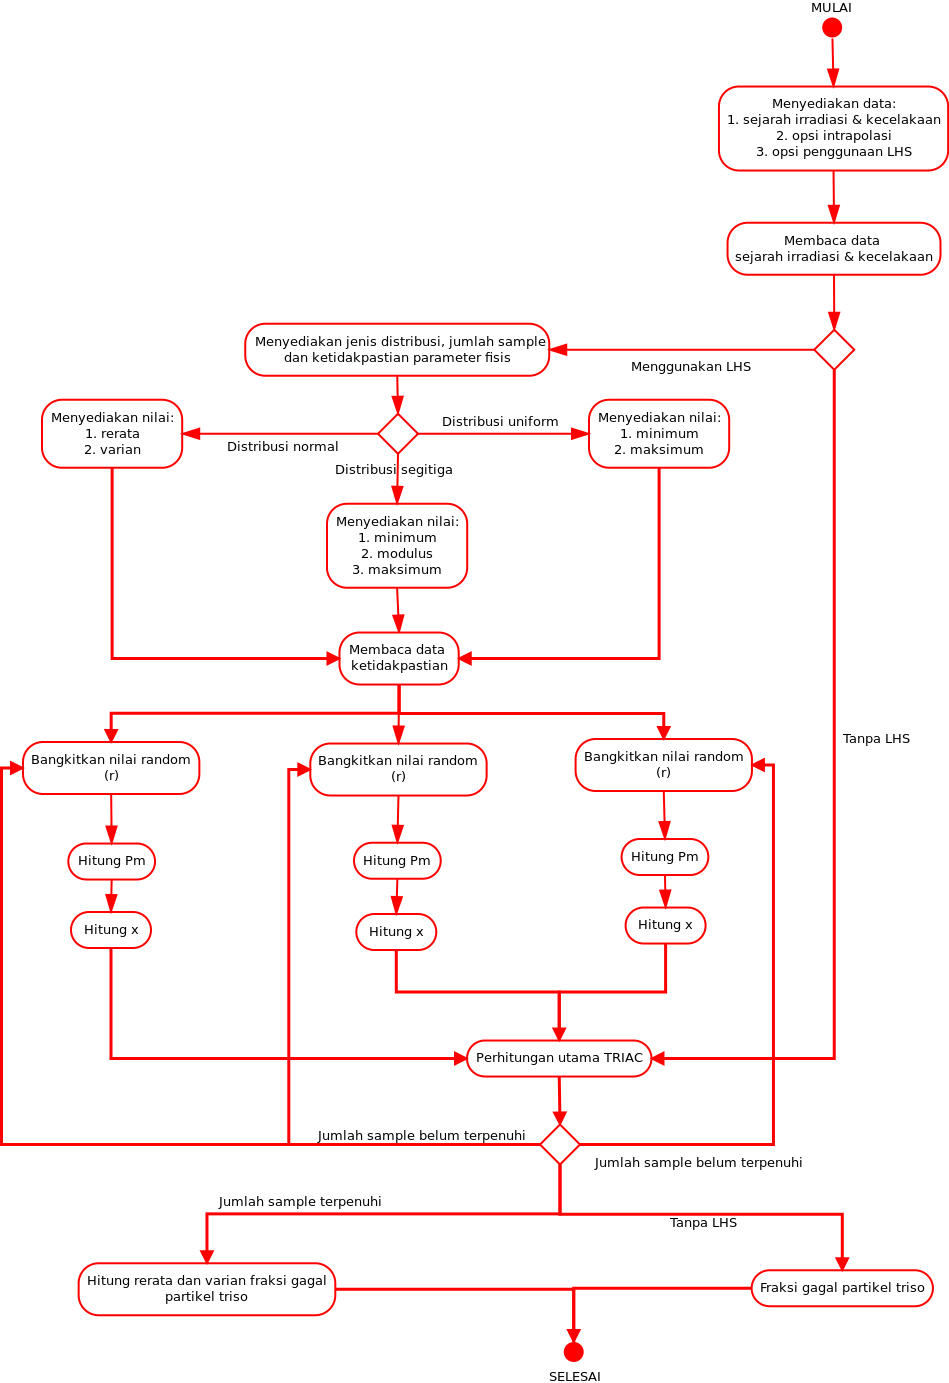
\includegraphics[scale=.45]{pics/aktifitasTotal.png}
    \caption{Diagram aktifitas eksekusi TRIAC}
    \label{fig:total}
  \end{center}
\end{figure}

\chapter{Penerapan TRIAC}
\label{sec:implementasitriac}
\section{Pendahuluan}
\label{sec:introPenerapan}
TRIA \textit{Code} yang telah dijelaskan sebelumnya secara umum dapat dikelompokkan menjadi dua tugas utama, masing-masing adalah perhitungan di waktu irradiasi dan kecelakaan. Saat irradiasi, hubungan saling ketergantungan antar variabel adalah seperti Gambar \ref{fig:irradiasi}. Sedangkan saat kecelakaan, hubungannya adalah seperti pada Gambar \ref{fig:accident}.

\begin{figure}[h]
  \begin{center}
    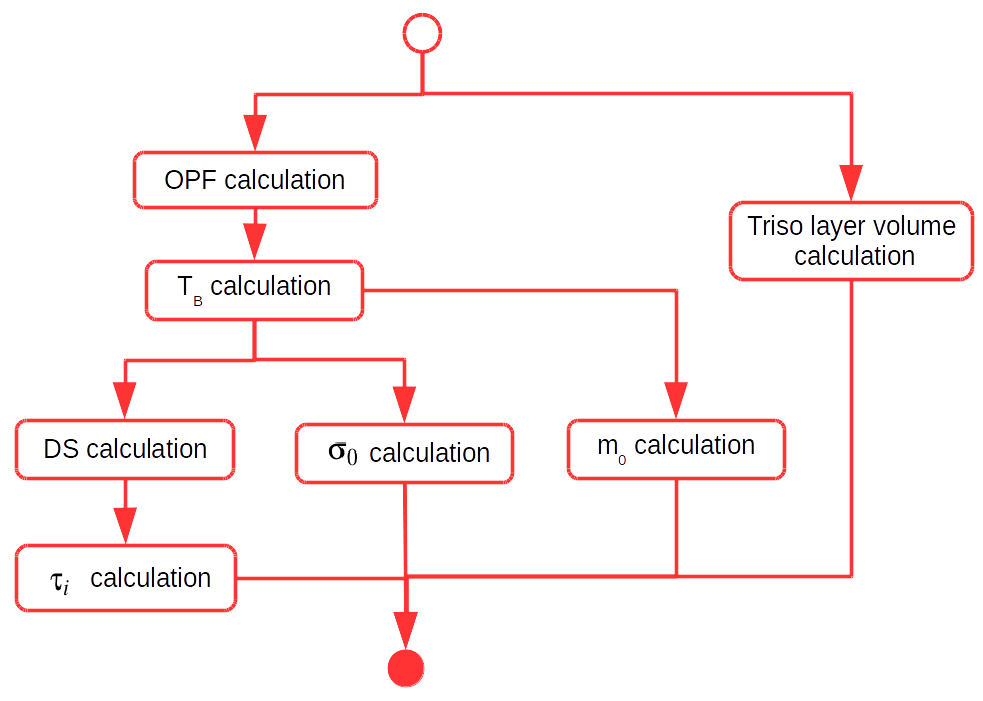
\includegraphics[scale=.5]{pics/irrCalculation.png}
    \caption{Hubungan ketergantungan antar variabel di fase irradiasi}
    \label{fig:irradiasi}
  \end{center}
\end{figure}

\begin{figure}[h]
  \begin{center}
    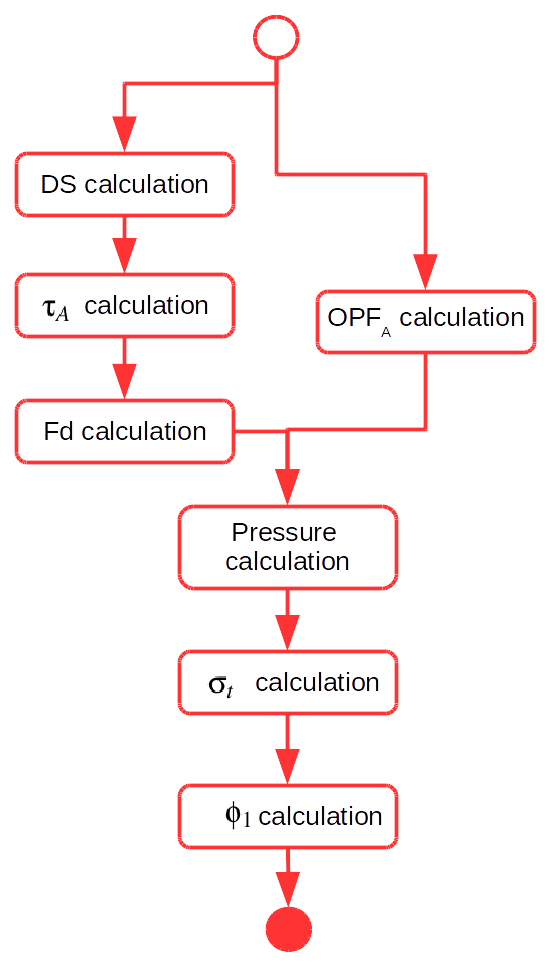
\includegraphics[scale=.5]{pics/accCalculation.png}
    \caption{Hubungan ketergantungan antar variabel di fase kecelakaan}
    \label{fig:accident}
  \end{center}
\end{figure}

Selanjutnya, triac juga memerlukan sejumlah data yang harus diberikan oleh pengguna sebelum perhitungan dimulai. Selain data-data seperti yang akan dijelaskan dalam sub bab \ref{sec:fileinput}, diperlukan juga beberapa data lain. Karena triac mengadopsi perhitungan yang dilakukan dalam PANAMA \cite{report1}, maka triac juga memerlukan data seperti yang diperlukan PANAMA. Tabel \ref{tab:additionalData} menyajikan beberapa parameter serta nilainya yang diperlukan oleh triac, masing untuk HTR-Modul dan HTR-500.

\begin{table}[h]
  \caption[Tambahan data yang diperlukan triac]{Tambahan data yang diperlukan triac\cite{report1}}
  \label{tab:additionalData}

  \begin{center}
  \ra{1.3}
    \begin{tabular}{@{}lrr@{}}\toprule
    %\hline
    Parameter & HTR-Modul & HTR-500 \\ \midrule%\hline
       Jenis partikel & $UO_2$ & $UO_2$ \\ 
       \textit{Burnup} / FIMA / $Fb$ & 0.08 & 0.08 \\
       \textit{Fast fluence} / $\Gamma$ [$10^{25}m^{-2}$] & 1.4 & 1.4 \\
       $\sigma_{oo}$ [MPa] & 834 & 834 \\
       $m_{oo}$ & 8.02 & 8.02 \\
       \bottomrule
    \end{tabular}
  \end{center}
\end{table}

Selain itu, triac juga memerlukan parameter lain berupa status interpolasi. Dengan status ini, sejarah irradiasi/kecelakaan akan diinterpolasi atau menggunakan nilai yang diberikan pengguna dari \textit{file input}.

\section{Pembacaan \textit{file input}}
\label{sec:fileinput}
Seluruh proses dalam triac didahului dengan membaca \textit{file input} dengan format yang sama seperti pada Lampiran \ref{lamp:inputExample}. Penerapan pembacaan \textit{file input} adalah seperti pada Listing \ref{InputData.py}.%\ref{triac.py}.

Di Listing \ref{InputData.py}, pembacaan \textit{input data} dilakukan secara sekuensial dan manual. Nilai-nilai yang harus dibaca ditentukan berdasarkan informasi yang ada pada \textit{file input}. Sebagai contoh, untuk membaca nilai geometri, digunakan karakter ''[m]'' sebagai penanda. Jika ditemukan karakter tersebut, maka di saat itulah pembacaan nilai geometri dilakukan. Hal inilah yang dimaksud sebagai pembacaan secara manual. Ketika karakter yang diperlukan berubah, maka modifikasi harus dilakukan pada modul ini.

Selain nilai terkait geometri, diperlukan juga pembacaan untuk nilai \textit{physical properties} serta sejarah operasi, baik saat operasi normal maupun kecelakaan. Pembacaan nilai yang berbeda dilakukan secara berurutan berdasarkan kemunculan nilai tersebut dalam \textit{file input}. Hal inilah yang dimaksud dengan pembacaan secara sekuensial.

Terdapat empat jenis data yang perlu dibaca dari \textit{file input} dalam Lampiran 1, masing-masing adalah sebagai berikut. Penerapannya disajikan dalam Listing \ref{InputData.py}.
\begin{enumerate}
  \item Data tentang geometri \textit{pebble}. Data ini diidentifikasi menggunakan teks yang didefinisikan oleh variabel \texttt{statusGeometry} (baris ke-4. Di dalam data geometri, terdapat empat data berbeda, masing-masing secara berurutan adalah panjang jejari \textit{pebble} terluar, OPyC (\textit{Outer Pyrolitic Carbon}), SiC (\textit{Silicon Carbide}), IPyC (\textit{Inner Pyrolitic Carbon}), \textit{buffer} dan kernel. Data geometri akan digunakan untuk menghitung volume setiap elemen pelapis (Gambar \ref{fig:bentukpebble}). Yang perlu diperhatikan adalah data jari-jari yang disajikan adalah jarak dari pusat bahan bakar sampai titik terluar dari setiap lapisan. Karena itu, volume suatu lapisan harus mempertimbangkan lapisan-lapisan di dalamnya. Data geometri disimpan dalam variabel diberi nama \texttt{dimensi} dan dalam bentuk \texttt{list} (baris ke-9).
  \item Data tentang kekuatan SiC. Data ini diidentifikasi menggunakan teks yang didefinisikan oleh variabel \texttt{statusCharacteristics} (baris ke-5 pada Listing \ref{InputData.py}). Ada empat nilai yang perlu dibaca terkait kekuatan SiC, masing-masing adalah SiC \textit{Tensile Strength} [Pa],	\textit{Weibull Modulus	Burnup} [FIMA],	\textit{Fission Yield of stable fission gasses} [Ff],	\textit{Fast Neutron Fluence}	dan rasio berat Th terhadap U-235 pada kernel. Data terkait kekuatan SiC disimpan dalam variabel yang diberi nama \texttt{characteristics} dalam bentuk \texttt{list} (baris ke-10).
    \item Data tentang sejarah irradiasi. Data ini diidentifikasi menggunakan teks yang didefinisikan oleh variabel \texttt{statusIrradiation} (baris ke-6 pada Listing \ref{InputData.py}). Data ini merupakan data temperatur bahan bakar \textit{pebble} pada selang waktu tertentu. Sebagai contoh, data yang disajikan pada Lampiran 1 diambil pada selang waktu 17 hari. Data sejarah irradiasi disimpan dalam variabel yang diberi nama \texttt{irradiation} dalam bentuk \texttt{list}. Setiap elemen adalah \texttt{list} yang secara \textit{nested} terdiri dari dua elemen yang mewakili data kolom kedua dan ketiga tiap akuisisi (baris ke-11). Ilustrasinya adalah seperti $[[0,	593], [1468800,	833], \ldots]$ dengan informasi waktu pengukuran dalam satuan detik. Data tentang nomor urut tidak digunakan karena selain tidak diperlukan dalam perhitungan, akan menyulitkan proses interpolasi yang akan diterapkan berikutnya.
    \item Data tentang sejarah kecelakaan. Data ini diidentifikasi menggunakan teks yang didefinisikan oleh variabel \texttt{statusAccident} (baris ke-7). Data ini memiliki pola yang sama dengan data sejarah irradiasi. Data sejarah keselakaan disimpan dengan cara yang sama seperti data tentang sejarah irradiasi tetapi dengan nama \texttt{accident} (baris ke-12). Ilustrasinya adalah seperti $[[0,	1033], [2341.44,	1033],\ldots]$ dengan informasi waktu pengukuran dalam satuan detik.
\end{enumerate}.

Namun, terlihat pada baris ke-76 dari Listing \ref{InputData.py}, terdapat total 5 variabel yang dikembalikan ke fungsi awal, dengan variabel kelima adalah $b-a$. Variabel ini adalah rentang waktu pengukuran data irradiasi.


Selain itu, untuk meningkatkan ketelitian perhitungan, disiapkan juga modul interpolasi secara linier. Modul ini disiapkan agar sejarah operasi normal dan kecelakaan sehingga dapat diperoleh hasil yang tepat. Penerapan dari modul interpolasi linier tersebut disajikan pada Listing \ref{Interpolasi.py}.

Seperti terlihat pada Lampiran \ref{lamp:inputExample}, sejarah operasi normal atau disebut juga sebagai sejarah irradiasi, terdapat 3 kolom dalam \textit{file input}. Demikian juga untuk sejarah ketika terjadi kecelakaan. Ketiganya adalah nomor urut, hari ke sekian dan temperatur. Dengan melakukan interpolasi, selisih hari yang digunakan dapat diperkecil. Dalam contoh \textit{file input}, selisih pencatatan adalah 17 hari. Dengan interpolasi, kita dapat mengestimasi sejarah dalam selisih waktu yang lebih singkat. 

Interpolasi yang diterapkan dapat diilustrasikan dalam Gambar \ref{fig:interpolasi} \footnote{\url{http://jadipaham.com/wp-content/uploads/2015/10/Rumus-interpolasi-linear.jpg}}. Argumen ketiga dari fungsi \texttt{linier (a,b,c)}, $c$, adalah jumlah partisi diantara nilai $x_1$ dan $x_2$. Nilai tersebut adalah $dt$ yang merupakan argumen ketika mengeksekusi kode komputer TRIAC (Listing \ref{triac.py}). Penggunaan fungsi interpolasi ini dilakukan di Listing \ref{triac.py} pada baris ke-53 s/d 66.

\begin{figure}
  \centering
  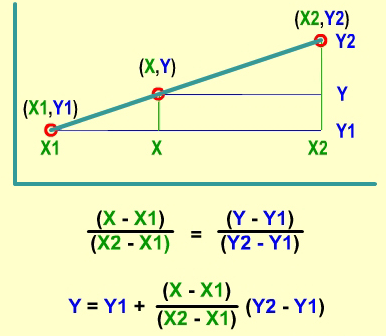
\includegraphics[scale=.5]{pics/interpolasi-linear.png}
  \caption{Ilustrasi interpolasi linier yang digunakan}
  \label{fig:interpolasi}
\end{figure}


\section{TRIAC Core}
Modul ini adalah modul yang diterapkan dalam bentuk \textit{class} seperti terlihat pada Listing \ref{core.py}. Modul ini dipersiapkan menjadi modul utama dalam TRIAC, baik ketika melibatkan perhitungan LHS maupun tidak.

Modul untuk perhitungan TRIAC dibuat dalam bentuk class yang menjalankan sejumlah fungsi dan menyimpan beberapa parameter dan konstanta yang diperlukan dalam perhitungan. Konstanta dan parameter diinisiasi dalam fungsi \texttt{\_\_init\_\_} serta dilengkapi sejumlah fungsi untuk memodifikasi nilainya. Berikut adalah konstanta dan parameter yang terlibat. Dari daftar tersebut, hanya \texttt{R} yang tidak memiliki fungsi modifikasi. Sedangkan \texttt{r} dan \texttt{d0} dimodifikasi melalui fungsi yang sama karena keduanya membutuhkan argumen yang sama. Yang selanjutnya masuk dalam kategori parameter adalah waktu (tb) dan temperatur irradiasi (Tb). Hal ini disebabkan karena parameter tersebut dihitung satu kali untuk kemudian digunakan dalam perhitungan fraksi gagal partikel triso di setiap \textit{mesh} waktu kecelakaan.
\begin{enumerate}
   \item \texttt{R}, konstanta gas, $8.3143 \left[\frac{J}{mole \cdot K}\right]$
   \item \texttt{Ff}, produk fisi yang dihasilkan dari gas fisi stabil
   \item \texttt{Fb}, \textit{burnup} logam berat / FIMA
   \item \texttt{Vm}, volume molar dalam partikel kernel yang dipengaruhi oleh material kernel,  $\left[\frac{m^3}{mole} \right]$
   \item \texttt{m00}, parameter weibull bahan bakar sebelum digunakan
   \item \texttt{r} (rerata jari-jari lapisan SiC) dan \texttt{d0} (ketebalan awal lapisan SiC)
   \item \texttt{sigma0}, \textit{tensile strength} SiC di akhir irradiasi [Pa]
   \item \texttt{Vk}, volume kernel [$m^3$]
   \item \texttt{Vf}, fraksi void, $0.5$ volume buffer.
   \item \texttt{tb}, waktu irradiasi, detik
   \item \texttt{Tb}, temperatur rerata irradiasi, $^{o}C$
   \item $\Gamma$, fluence neutron cepat, $10^{25} m^{-2} $ EDN
 \end{enumerate} 

Sedangkan daftar fungsi yang terdapat dalam class \texttt{Core} adalah sebagai berikut.
\begin{enumerate}
  \item Perhitungan volume lapiran triso.
  \begin{itemize}
    \item Nama fungsi: \texttt{volume}
    \item Argumen: \texttt{radius} (jari-jari lapisan partikel triso) 
    \item Formula yang dikerjakan: $v=\frac{4}{3}\;\pi\;radius^2$
    \item \textit{Return value}: \texttt{v}
  \end{itemize}
  \item OPF (\textit{Oxygen Per Fission})
  \begin{itemize}
    \item Nama fungsi: \texttt{OPF}
    \item Argumen: \texttt{irradiation,y}
    \begin{itemize}
      \item \texttt{irradiation}: \textit{array} berdimensi dua, dengan kolom pertama adalah waktu dengan satuan detik sedangkan kolom kedua adalah temperatur dengan satuan $^{o}C$
      \item \texttt{y}: rentang waktu pengukuran sejarah irradiasi dengan satuan detik. Dikaitkan dengan argumen \texttt{irradiation}, maka \texttt{y} adalah rentang waktu antara dua waktu berurutan di dalamnya.
    \end{itemize}
    \item Formula yang dikerjakan: Listing \ref{OPF}
    \item \textit{Return value}: \texttt{z}
    
\scriptsize
\begin{lstlisting}[language=python, numbers=left, numberstyle=\tiny, caption=Fungsi OPF, showstringspaces=false, label=OPF]
def OPF(self,irradiation,y):
	x=len(irradiation)
	print("Irradiation length:",x)
	z=0.0
	for i in range(x):
		j=irradiation[i]
		a1=self.R*j[1]
		a=-163000/(a1)
		b=math.exp(a)
		g=2*(8.32e-11)*b
		g1=g*(self.tb-j[0])*y
		z=z+g1
  return z
\end{lstlisting}
\normalsize
  \end{itemize}
  \item $F_{\tau}$
  \begin{itemize}
    \item Nama fungsi: \texttt{FTau}
    \item Argumen: \texttt{tau}, salah satu parameter dalam sejumlah formula empiris pada PANAMA \cite{report1}
    \item Formula yang dikerjakan: Listing \ref{FTau}
    \item \textit{Return value}: \texttt{ftau}
    
\scriptsize
\begin{lstlisting}[language=python, numbers=left, numberstyle=\tiny, caption=Fungsi FTau, showstringspaces=false, label=FTau]    
def FTau(self,tau):
	looping=0.0
	for n in range (1,2000):
		pangkat=math.pow(n,2)*math.pow(math.pi,2)*tau
		A=math.exp(-(pangkat))
		B=math.pow(n,4)*math.pow(math.pi,4)
		looping=looping+((1-A)/B)			
	ftau=1-((6/tau)*looping)
	return ftau
\end{lstlisting}
\normalsize
    
  \end{itemize}
  \item DS
  \begin{itemize}
    \item Nama fungsi: \texttt{DS}
    \item Argumen: \texttt{T}, temperatur dalam $^{o}C$
    \item Formula yang dikerjakan: Listing \ref{DS}
    \item \textit{Return value}: \texttt{ds}
    
\scriptsize
\begin{lstlisting}[language=python, numbers=left, numberstyle=\tiny, caption=Fungsi DS, showstringspaces=false, label=DS]
def DS(self,T):
	logDS=-2.3-(8116/T)
	ds=math.pow(10,logDS)
	return ds
\end{lstlisting}
\normalsize

  \end{itemize}
  \item OPF Accident
  \begin{itemize}
    \item Nama fungsi: \texttt{OPFAccident}
    \item Argumen:
    \begin{itemize}
      \item \texttt{T}: temperatur ketika terjadi kecelakaan, $^{o}C$
    \end{itemize}
    \item Formula yang dikerjakan: Listing \ref{OPFAccident}
    \item \textit{Return value}: \texttt{opfa}
    
\scriptsize
\begin{lstlisting}[language=python, numbers=left, numberstyle=\tiny, caption=Fungsi OPFAccident, showstringspaces=false, label=OPFAccident]
def OPFAccident(self,T):	
	logOPF=-10.08-(8500/self.Tb)+(2*math.log10(self.tb))-
	(0.404*((10000/T)-(10000/(self.Tb+75))))
	opfa=math.pow(10,logOPF)
	return opfa
\end{lstlisting}
\normalsize
  \end{itemize}

  \item Parameter weibull
  \begin{itemize}
    \item Nama fungsi: \texttt{weibullParam}
    \item Argumen:
    \begin{itemize}
      \item \texttt{T}: temperatur ketika terjadi kecelakaan, $^{o}C$
      \item \texttt{t}: waktu ketika terjadi kecelakaan, detik 
    \end{itemize}
    \item Formula yang dikerjakan: Listing \ref{weibull}
    \item \textit{Return value}: \texttt{m}
    \item Catatan: pada penerapannya, perhitungan ini tidak dilakukan. Jika dilibatkan dalam perhitungan, maka fraksi gagal partikel triso akan lebih besar daripada hasil yang diperoleh PANAMA. Meskipun hal itu logis, karena temperatur yang lebih tinggi akan meningkatkan potensi kerusakan partikel triso, tetapi tahap awal pengembangan TRIAC mentargetkan sedekat mungkin hasil yang diperoleh dengan PANAMA. Karena itu, diasumsikan bahwa parameter weibull tidak berubah selama kecelakaan terjadi. Seperti terlihat pada Listing \ref{core.py}, fungsi untuk menghitung parameter weibull terkini tidak dijalankan, dan hanya bertugas mengembalikan nilai parameter, tepat saat dimulainya kecelakaan ($m_0$).
    
\scriptsize
\begin{lstlisting}[language=python, numbers=left, numberstyle=\tiny, caption=Fungsi weibullParam, showstringspaces=false, label=weibull]
def weibullParam(self,T,t):
	logGammaM=0.394+(650/self.Tb)
	gammaM=math.pow(10,logGammaM)
	m0=self.m00*(1-(self.Fluence/gammaM))
	a=-187400/(self.R*T)
	b=math.pow(math.e,a)
	etaDot=0.565*b
	c=math.pow(math.e,-etaDot*t)
	m=m0*(0.44+(0.56*c))
	return m
\end{lstlisting}
\normalsize
  \end{itemize}
  
  \item tekanan
  \begin{itemize}
    \item Nama fungsi: \texttt{tekanan}
    \item Argumen:
    \begin{itemize}
      \item \texttt{Fd}: fraksi gas fisi yang lepas
      \item \texttt{opf}: \textit{oxygen per fission} saat terjadi kecelakaan
      \item \texttt{T}: temperatur ketika terjadi kecelakaan, $^{o}C$
    \end{itemize}
    \item Formula yang dikerjakan: Listing \ref{tekanan}
    \item \textit{Return value}: \texttt{p}
    
\scriptsize
\begin{lstlisting}[language=python, numbers=left, numberstyle=\tiny, caption=Fungsi tekanan, showstringspaces=false, label=tekanan]
def tekanan(self,Fd,opf,T):
	p=((Fd*self.Ff)+opf)*self.Fb*(self.Vk/self.Vm)*self.R*T/self.Vf
	return p
\end{lstlisting}
\normalsize
  \end{itemize}
  
  \item $\sigma_T$
  \begin{itemize}
    \item Nama fungsi: \texttt{sigmaT}
    \item Argumen:
    \begin{itemize}
      \item \texttt{p}: tekanan (Pa)
      \item \texttt{t}: waktu terjadi kecelakaan, detik
      \item \texttt{T}: temperatur ketika terjadi kecelakaan, $^{o}C$
    \end{itemize}
    \item Formula yang dikerjakan: Listing \ref{sigmaT}
    \item \textit{Return value}: \texttt{a}
    
\scriptsize
\begin{lstlisting}[language=python, numbers=left, numberstyle=\tiny, caption=Fungsi \textit{tensile strength} pada temperatur T, showstringspaces=false, label=sigmaT]
	def SIGMA_T(self,p,t,T):
		nu=(5.87e-7)*math.exp(-179500/(self.R*T))
		a=(self.r*p/(2*self.d0))*(1+(nu*t/self.d0))
		return a
\end{lstlisting}
\normalsize
  \end{itemize}
  
  \item $\phi$
  \begin{itemize}
    \item Nama fungsi: \texttt{phi}
    \item Argumen:
    \begin{itemize}
      \item \texttt{sigmaT}: \textit{tensile strength} pada temperatur \texttt{T}
      \item \texttt{m}: parameter weibull
    \end{itemize}
    \item Formula yang dikerjakan: Listing \ref{phi}
    \item \textit{Return value}: \texttt{d}
    
\scriptsize
\begin{lstlisting}[language=python, numbers=left, numberstyle=\tiny, caption=Fungsi fraksi gagal partikel triso, showstringspaces=false, label=phi]
	def PHI(self,sigmaT, m):
		a=sigmaT/self.sigma0
		b=math.pow(a,m)
		c=math.log(2)*b
		d=1-math.exp(-c)
		return d
\end{lstlisting}
\normalsize
  \end{itemize}
\end{enumerate}



\section{Perhitungan TRIAC}
Bagian ini adalah bagian pengendali dari perhitungan TRIAC yang alur eksekusinya diilustrasikan pada Gambar \ref{fig:flowchart}. Sedangkan hubungan interaksi antar fungsi untuk mendapatkan nilai fraksi gagal partikel triso setelah sekian waktu sejak terjadi kecelakaan dapat diilustrasikan seperti Gambar \ref{fig:interaksiformula}. Kotak dengan warna merah, kuning dan hijau pada Gambar \ref{fig:interaksiformula} menunjukkan formula-formula yang hasilnya menjadi masukan untuk formula pada kotak berwarna biru. Sementara angka di bawah kotak-kotak tersebut adalah nomor formula dalam dokumen PANAMA \cite{report1}.

\begin{figure}[h]
  \begin{center}
    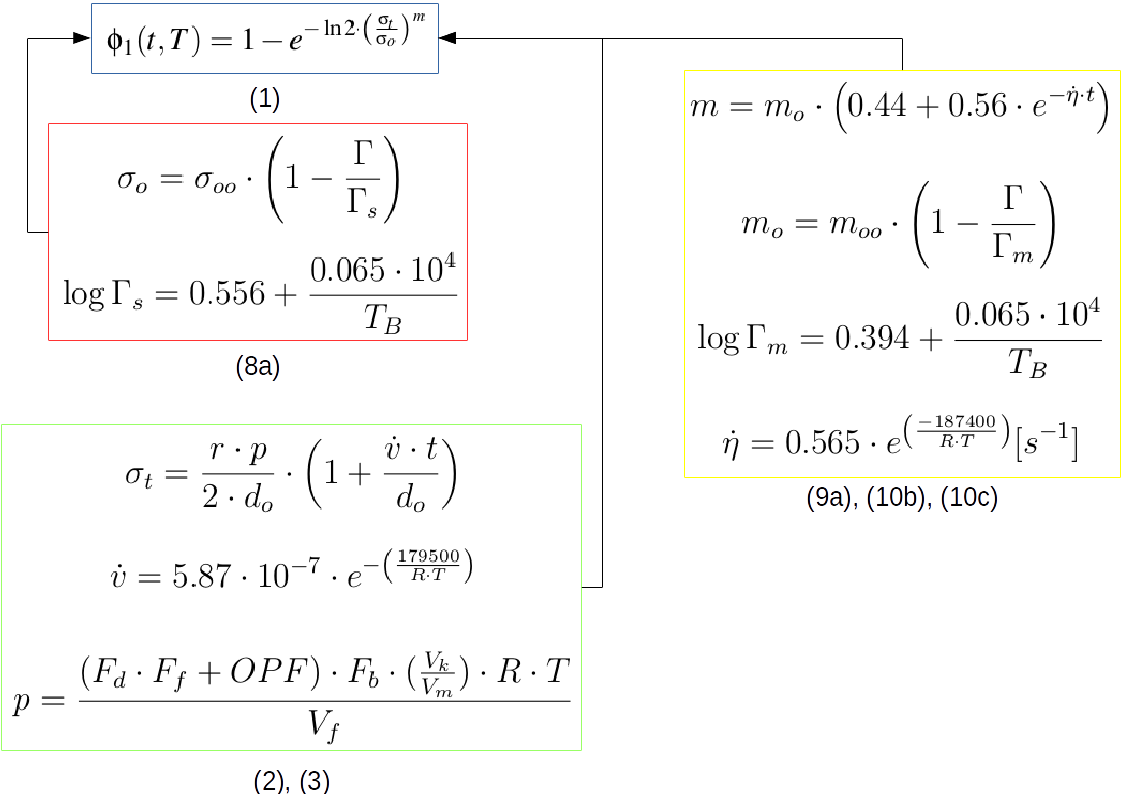
\includegraphics[scale=.5]{pics/alurRumus1.png}
    \caption{Interaksi antar fungsi untuk mendapatkan fraksi gagal partikel triso}
    \label{fig:interaksiformula}
  \end{center}
\end{figure}


Sedangkan Gambar \ref{fig:interaksiformula2} merupakan kelanjutan dari interaksi yang ditunjukkan Gambar \ref{fig:interaksiformula}, khususnya untuk menyediakan nilai masukan bagi parameter nilai tekanan yang dialami lapisan silikon karbida. Sama seperti Gambar \ref{fig:interaksiformula}, angka di bawah kotak-kotak berwarna yang berisi formula pada Gambar \ref{fig:interaksiformula2} menunjukkan nomor formula pada dokumen PANAMA \cite{report1}. Selain informasi nomor persamaan pada dokumen PANAMA, ditunjukkan pula bahwa kotak berwarna kuning merupakan variabel yang dipengaruhi oleh jenis partikel triso. Formula yang disajikan merupakan formula empiris untuk jenis partikel $UO_2$. Sementara untuk kotak berwarna hijau, selain dipengaruhi oleh jenis material partikel triso, juga dipengaruhi oleh kondisi apakah partikel triso sedang berada pada masa irradiasi (formula pertama) atau kecelakaan (formula kedua). 

%Dari Gambar \ref{fig:interaksiformula} dan \ref{fig:interaksiformula2} 

\begin{figure}[h]
  \begin{center}
    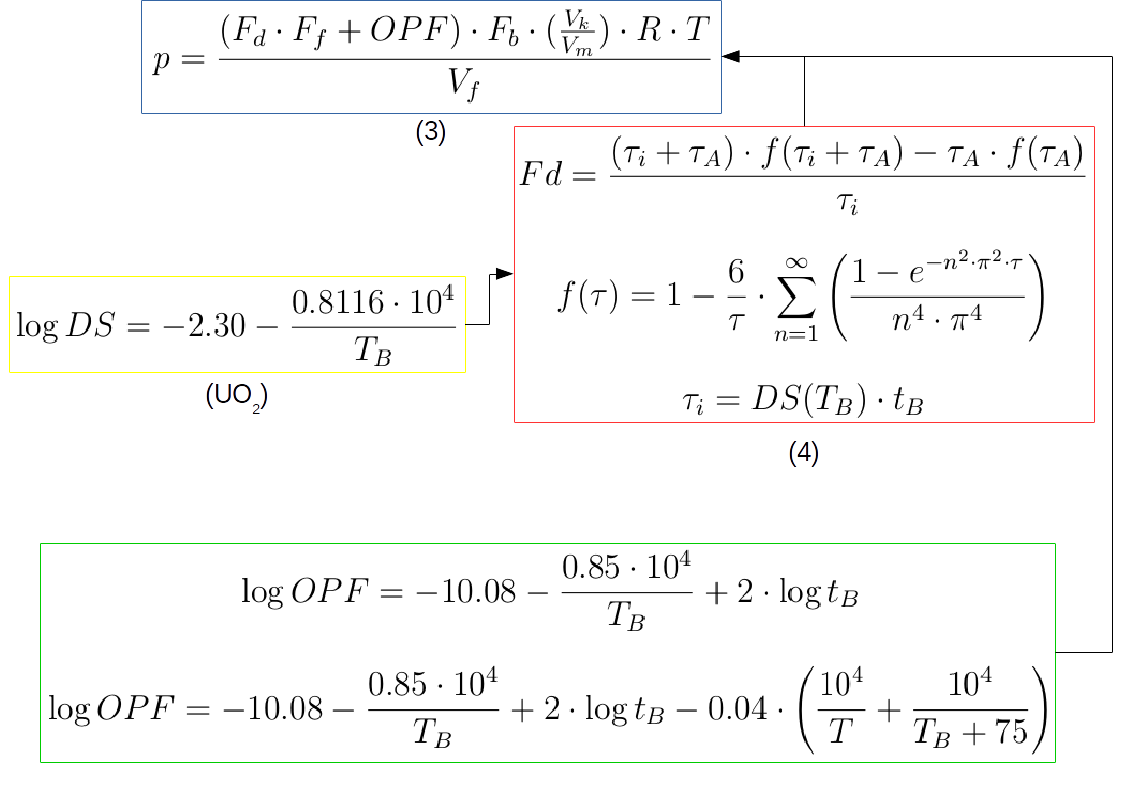
\includegraphics[scale=.5]{pics/alurRumus2.png}
    \caption{Interaksi antar fungsi untuk mendapatkan nilai tekanan yang dialami lapisan silikon karbida}
    \label{fig:interaksiformula2}
  \end{center}
\end{figure}

Program ini dirancang untuk dapat menerima tiga kombinasi argumen, masing-masing adalah eksekusi TRIAC tanpa perhitungan LHS, dengan LHS dan tanpa argumen yang berarti telah ada \textit{file input} yang terdefinisi lengkap dengan tambahan untuk \textit{meshing} interpolasi.

Proses selanjutnya adalah membaca informasi dari \textit{file input}. Ada lima informasi yang harus diperoleh dari \textit{file input}, masing-masing adalah informasi geometri, karakteristik material, sejarah irradiasi dan kecelakaan serta rentang pengukuran temperatur saat irradiasi. Setelah data-data tersebut diperoleh, langkah selanjutnya adalah perhitungan geometri partikel triso. Kemudian, agar perhitungan dapat dilakukan, perlu dilakukan inisiasi obyek dari \textit{class} \texttt{core.py}. Setelah obyek tersebut diinisiasi, semua perhitungan seperti ditunjukkan dalam Gambar \ref{fig:flowchart} dilakukan.

Seperti telah dijelaskan dalam sub bab \ref{sec:introPenerapan}, TRIAC menjalankan perhitungan pada kondisi irradiasi (Gambar \ref{fig:irradiasi}) dan kecelakaan (Gambar \ref{fig:accident}). Perhitungan pada kondisi irradiasi akan menghasilkan $T_B$ yang secara bertahap diperoleh dari \textit{mesh} sejarah irradiasi kemudian $OPF$. Selanjutnya, nilai $T_B$ akan digunakan untuk menghitung $\tau_i$, $\sigma_0$ dan $m_0$. Kemudian, perhitungan di kondisi irradiasi juga menghasilkan volume setiap layer dalam partikel triso, khususnya volume dua lapisan terdalam (kernel dan buffer, lihat Gambar \ref{fig:bentukpebble}). Nilai-nilai tersebut digunakan dalam perhitungan ketika kondisi kecelakaan terjadi, hingga akhirnya diketahui fraksi gagal partikel triso. 

Yang menarik adalah model yang dikembangkan oleh PANAMA di kondisi kecelakaan yang melakukan perhitungan semua parameter di setiap \textit{mesh} sejarah kecelakaan. Hal ini berbeda ketika perhitungan dilakukan di kondisi irradiasi, hanya diperoleh nilai antara untuk selanjutnya diperoleh hasil akhir berupa $T_B$. Dari $T_B$ inilah nantinya diperoleh $\tau_i$, $\sigma_0$ dan $m_0$. Kondisi ini sejalan dengan model pertumbuhan fraksi gagal $\phi_1$ yang selalu mengacu pada kondisi awal kecelakaan (akhir irradiasi). Seperti ditunjukkan di Gambar \ref{fig:interaksiformula2}, selalu ada parameter $T_B$, $\tau_i$ dalam perhitungan nilai OPF kecelakaan, $Fd$ dan tekanan internal ($p$). Juga $\sigma_0$ dan $m_0$ dalam perhitungan $\sigma_t$ dan $\phi_1$ (Gambar \ref{fig:accident}).

\chapter{Pengujian perhitungan TRIAC}
\section{Pendahuluan}
Pengujian dilakukan dengan membandingkan hasil perhitungan TRAIC dengan PANAMA untuk data \textit{file input} seperti dalam Lampiran \ref{lamp:inputExample}. Khusus untuk hasil PANAMA, hanya terdapat hasil plot kondisi pengujian yang terdapat dalam dokumen teknis \cite{report1} (Gambar \ref{fig:benchmark1}). Dari gambar tersebut, direkonstruksi titik-titik hubungan antara waktu (jam) di sumbu (x) terhadap $\phi_1$ di sumbu (y). Karena itu, hasil pengujian TRIAC akan sangat tergantung dengan ketelitian dalam merekonstruksi titik tersebut. Pengujian yang dilakukan telah disajikan dalam artikel \cite{triac}.

\begin{figure}[h!]
  \begin{center}
    \includegraphics[scale=.45]{pics/benchmarkPANAMA.png}
    \caption[Hasil perhitungan PANAMA untuk berbagai kondisi pengujian]{Hasil perhitungan PANAMA untuk berbagai kondisi pengujian \cite{report1}}
    \label{fig:benchmark1}
  \end{center}
\end{figure}

\section{Hasil pengujian}
Seperti ditunjukkan Gambar \ref{fig:benchmark1}, kondisi pengujian adalah sebagai berikut. Hasilnya ditunjukkan pada Gambar \ref{fig:compareinit}.
\begin{enumerate}
  \item Kondisi kecelakaan DLOFC (\textit{Depressurized Loss Of Forced Cooling}) seperti kondisi \textit{mesh} sejarah kecelakaan yang sama dengan data di Lampiran \ref{lamp:inputExample}
  \item Kondisi DLOFC dengan \textit{mesh} sejarah kecelakaan sebelumnya ditambah $100^o$C
  \item Kondisi \textit{mesh} sejarah kecelakaan yang stabil di angka $1600^o$C
\end{enumerate}

\begin{figure}[h!]
  \begin{center}
    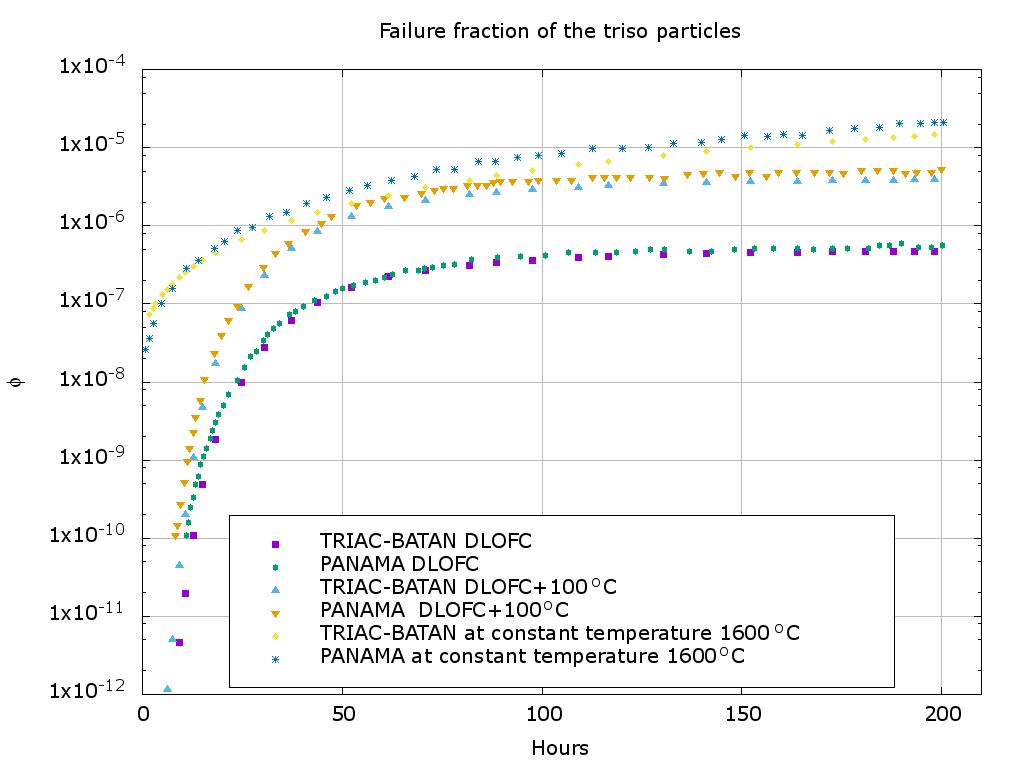
\includegraphics[scale=.35]{pics/compareinit.png}
    \caption{PANAMA vs. TRIAC-BATAN for three accident scenarios}
    \label{fig:compareinit}
  \end{center}
\end{figure}

\chapter{Penerapan modul \textit{sampling}}
\section{Pendahuluan}
\label{sec:introsampling}
Modul sampling yang akan diintegrasikan dalam TRIAC memiliki struktur class seperti pada Gambar \ref{fig:samplingclass}. Setiap distribusi menerapkan perhitungannya masing-masing untuk mendapatkan variabel sampling. Sedangkan class \texttt{triacLHS} sebagai super class menangani semua layanan lain yang berlaku untuk semua distribusi.

\begin{figure}[h]
  \begin{center}
    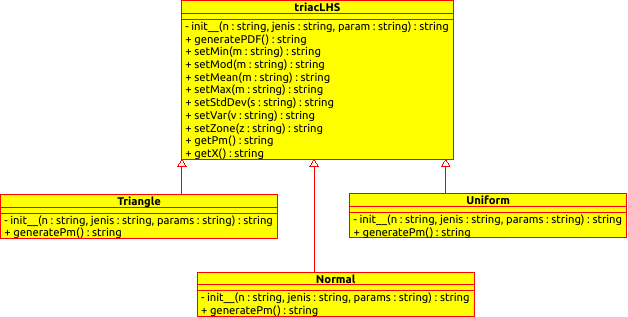
\includegraphics[scale=.75]{pics/samplingclass.png}
    \caption{Keterkaitan antar class dalam modul \textit{sampling}}
    \label{fig:samplingclass}
  \end{center}
\end{figure}

Dengan struktur TRIAC yang telah dibangun sebelumnya (Bab \ref{sec:implementasitriac}), diperlukan alur eksekusi yang dapat mengintegrasikan keduanya seperti yang disajikan di Gambar \ref{fig:total}. Selanjutnya, agar dapat diterapkan diperlukan skenario eksekusi layanan antar class seperti yang ditunjukkan pada Gambar \ref{fig:sequence}. Dalam Gambar \ref{fig:sequence}, class \texttt{LHSCalculation} berperan sebagai antarmuka untuk memanfaatkan layanan yang disediakan modul \textit{sampling}. Melalui class \texttt{LHSCalculation}, argumen yang diberikan oleh pengguna seperti jumlah \textit{sample} yang dibutuhkan, jenis distribusi dan \textit{sampling}, layer triso mana saja yang perlu di-\textit{sampling} disampaikan ke modul \textit{sampling}. Class \texttt{LHSCalculation} juga menjadi perantara untuk \textit{sample} dihasilkan dan selanjutnya dikembalikan ke TRIAC.

\begin{figure}[h]
  \begin{center}
    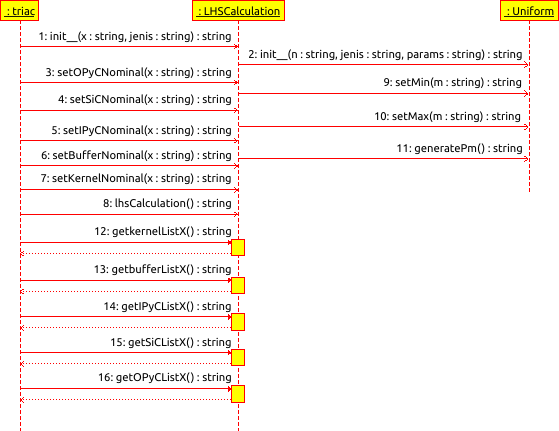
\includegraphics[scale=.75]{pics/sequencediagram.png}
    \caption{Diagram \textit{sequence} eksekusi layanan antar class yang melibatkan modul \textit{sampling}}
    \label{fig:sequence}
  \end{center}
\end{figure}

Jenis data \texttt{string} yang terlihat dalam rangkaian eksekusi layanan di Gambar \ref{fig:sequence} adalah hasil transformasi kode sumber python oleh aplikasi UML modeler, Umbrello \footnote{\url{https://umbrello.kde.org/}}. Meskipun umumnya berupa list yang berisi informasi ketidakpastian pada lapisan triso. Informasi ketidakpastian yang akan digunakan dalam pengujian TRIAC dengan modul \textit{sampling} diberikan pada Tabel \ref{tab:uncertainty}. 

Informasi terkait ketidakpastian tersebut dimasukkan ke TRIAC melalui \textit{file input} seperti pada Lampiran \ref{lamp:inputExample}, di bawah baris informasi ''Uncertainties in geometry and a number of samples:''. Untuk setiap layer, terdapat 3 nilai yang harus diberikan, masing-masing adalah nilai ketidakpastian, jenis distribusi serta standar deviasi ($\sigma$) jika jenis distribusi yang dipilih adalah normal. Jika jenis distribusi yang dipilih bukan normal, maka nilai $\sigma$ diisi dengan $0$. Demikian juga jika lapisan triso tertentu, atau bahkan semuanya, tidak dipertimbangkan ketidakpastiannya, di bagian itu diisi nilai $0$. Sementara nilai terakhir di barisan itu adalah jumlah \textit{sample}. Modul sampling ini menerapkan kebijakan untuk menggunakan jumlah \textit{sample} yang sama untuk semua layer triso.

\begin{sidewaystable}[h]
\caption{Nilai nominal dan ketidakpastiannya pada lapisan triso}
\label{tab:uncertainty}
  \begin{center}
    \begin{tabular}{@{}cccccccccccccc@{}}\toprule[1.5pt]
    %\hline
     \multicolumn{2}{c}{OPyC} & \phantom{a} & \multicolumn{2}{c}{SiC} & \phantom{a} & \multicolumn{2}{c}{IPyC} & \phantom{a} & \multicolumn{2}{c}{Buffer} & \phantom{a} & \multicolumn{2}{c}{Kernel}\\ \cmidrule{1-2} \cmidrule{4-5} \cmidrule{7-8} \cmidrule{10-11} \cmidrule{13-14}
     Nominal & Ketidakpastian && Nominal & Ketidakpastian && Nominal & Ketidakpastian && Nominal & Ketidakpastian && Nominal & Ketidakpastian\\ \midrule
     $4.60^{-4}$ & $1.0^{-5}$ && $4.20^{-4}$ & $2.6^{-6}$ && $3.85^{-4}$ & $1.0^{-5}$ && $3.45^{-4}$ & $4.4^{-6}$ && $2.55^{-4}$ & $5.0^{-6}$\\
       \bottomrule[1.5pt]
    \end{tabular}
  \end{center}
\end{sidewaystable}

Kembali ke Gambar \ref{fig:total}, penggunaan modul \textit{sampling} akan membuat perhitungan TRIAC melakukan perulangan sebanyak jumlah \textit{sample}. Tentunya setelah sample telah dihasilkan oleh modul \textit{sampling}. Karena ada sebanyak jumlah \textit{sample} kombinasi ketebalan lapisan triso, maka akan ada sebanyak itu pula hasil perhitungan fraksi gagal triso. Itu sebabnya, di akhir perhitungan yang dijelaskan dalam diagram aktifitas di Gambar \ref{fig:total} ada perhitungan rerata dan variance dari nilai fraksi gagal yang ada sebanyak jumlah \textit{sample}.
\clearpage
\section{Pembacaan \textit{file input}}
\label{sec:inputlhs}
Pembacaan informasi terkait ketidakpastian ketebalan lapisan triso dilakukan di kode yang sama seperti informasi lainnya (Listing \ref{InputData.py}). Seperti telah dijelaskan di Sub bab \ref{sec:introsampling}, setiap lapisan partikel triso akan memiliki 3 data, masing-masing adalah ketidakpastian, jenis distribusi \textit{sample} dan $\sigma$. Ketiga data tersebut kemudian disusun dalam 1 list. List berisi data ketidakpastian setiap layer selanjutnya digabungkan dengan data sejenis dari layer yang lain. Sedangkan jumlah \textit{sample} yang terlibat menjadi data yang terakhir yang disimpan dalam list utama yang diberi nama \texttt{uncertainties} (baris ke-63 di Listing \ref{InputData.py}).

\section{Trigger ke modul \textit{sampling}}
Seperti telah dijelaskan pada Gambar \ref{fig:sequence}, permintaan layanan pada modul \textit{sampling} dilakukan dari class \texttt{triac.py} (baris ke-224 dari Listing \ref{triac.py}). Terdapat 2 argumen yang harus disertakan saat melakukan inisiasi obyek \texttt{LHSCalculation}. Keduanya adalah data ketidakpastian yang diperoleh dari pembacaan \textit{file input} (sub bab \ref{sec:inputlhs}) serta informasi tentang apakah akan menggunakan metode \textit{sampling} LHS atau SRS.

Argumen yang dilewatkan ke \texttt{LHSCalculation} akan dipecah dan dimasukkan ke variabel yang bersesuaian. Sebagai contoh, elemen pertama dari list \texttt{uncertainties} adalah data ketidakpastian dari lapisan OPyC. Demikian untuk selanjutnya. Kondisi ini dapat dilihat pada fungsi \texttt{\_\_init\_\_} pada \texttt{LHSCalculation} di Listing \ref{LHScalculation.py}. 

Setelah inisiasi obyek \texttt{LHSCalculation}, \texttt{triac.py} selanjutnya memasukkan nilai nominal dari ketebalan seluruh lapisan triso. Proses ini dijelaskan dalam Gambar \ref{fig:sequence} sebagai pemanggilan fungsi ke-3,4,5,6 dan 7, masing-masing untuk lapisan OPyC, SiC, IPyC, buffer dan kernel. 

Kemudian, jika distribusi yang dipilih adalah \textit{uniform} maka \texttt{LHSCalculation} harus memasukkan nilai minimum dan maksimum dari rentang ketidakpastian. \texttt{LHSCalculation} mengetahui apa yang harus dilakukan karena sebelumnya, \texttt{triac.py} menjalankan perintah \texttt{lhsCalculation} (baris ke-235 pada Listing \ref{triac.py}). Perintah tersebut akan menjalankan layanan yang tersedia di \texttt{LHSCalculation}, tepatnya layanan yang didefinisikan pada baris ke-93 pada Listing \ref{LHScalculation.py}. Di dalam layanan tersebutlah, ditentukan inisiasi obyek lhs, apakah dari clas \texttt{Uniform}, \texttt{Triangle} ataupun \texttt{Normal}. Setelah penentuan obyek tersebut, pemberian nilai awal dilakukan, yang dalam Gambar \ref{fig:sequence} dilakukan pada pemanggilan fungsi ke-9 dan 10. Setiap obyek distribusi akan memiliki nilai awal yang berbeda. Hal ini menyebabkan definisi dari layanan \texttt{lhsCalculation} cukup panjang untuk mengakomodasi semua opsi yang mungkin.

Layanan terakhir yang pada Gambar \ref{fig:sequence} dijalankan oleh LHSCalculation adalah \texttt{generatePm}. Meskipun bernama sama, penerapannya berbeda-beda dari satu distribusi ke distribusi lainnya. Karena itu, penerapannya dilakukan di class distribusi. Hasil dari pemanggilan fungsi ini adalah \textit{sample} dengan kriteria jumlah dan distribusi seperti yang diinginkan. Setelah layanan tersebut selesai, obyek \texttt{triac} dapat menggunakan \textit{sample} tersebut untuk menghitung fraksi gagal triso. Selesainya layanan tersebut ditandai dengan pengambilan \textit{sample} oleh obyek \texttt{triac} dari \texttt{LHSCalculation}. Pengambilan sample tersebut dalam Gambar \ref{fig:sequence} direpresentasikan oleh pemanggilan fungsi ke-12 s/d 16.

\chapter{Pengujian modul \textit{sampling}}
\section{Pendahuluan}
Pengujian modul sampling akan mengunakan data sejarah irradiasi dan kecelakaan yang sama dengan yang telah digunakan pada pengujian perhitungan utama TRIAC. Sedangkan data ketidakpastian adalah seperti Tabel \ref{tab:uncertainty}. Pengujian diawali dengan membuat sample dengan mengikuti distribusi tertentu. Dalam hal ini adalah distribusi \textit{uniform} dan triangular. Sedangkan modul untuk distribusi normal yang telah diimplementasikan masih menghasilkan pola yang berbeda dari yang seharusnya. Jika telah dapat terbentuk, maka pengunaannya akan sama seperti modul dengan distribusi \textit{uniform} dan triangular.

\section{Hasil pengujian}
Pengujian pertama adalah membentuk sample sehingga memiliki distribusi tertentu, baik menggunakan metode LHS dan SRS. Gambar \ref{fig:unifLHS} dan \ref{fig:unifSRS} menunjukkan \textit{sample} yang terbentuk mengikuti distribusi \textit{uniform}, dengan menggunakan metode LHS dan SRS. Sedangkan Gambar \ref{fig:triLHS} dan \ref{fig:triSRS} menunjukkan pola serupa dengan distribusi triangular. Terlihat bahwa metode LHS dapat membentuk sample yang jumlahnya terdistribusi dengan distribusi tertentu. Sedangkan SRS, cukup acak dalam distribusinya.

\begin{figure}[h!]
\begin{center}
\subfigure[]{\label{fig:unifLHS}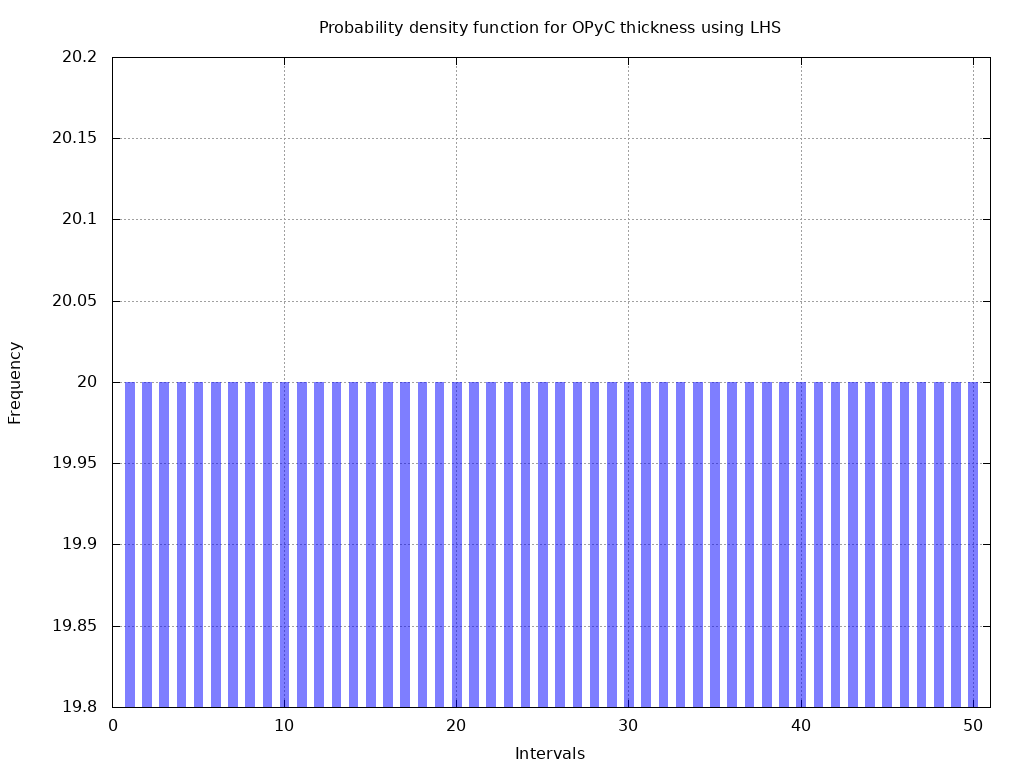
\includegraphics[width=130mm]{pics/LHS_Uniform_OPyC.png}}
\subfigure[]{\label{fig:unifSRS}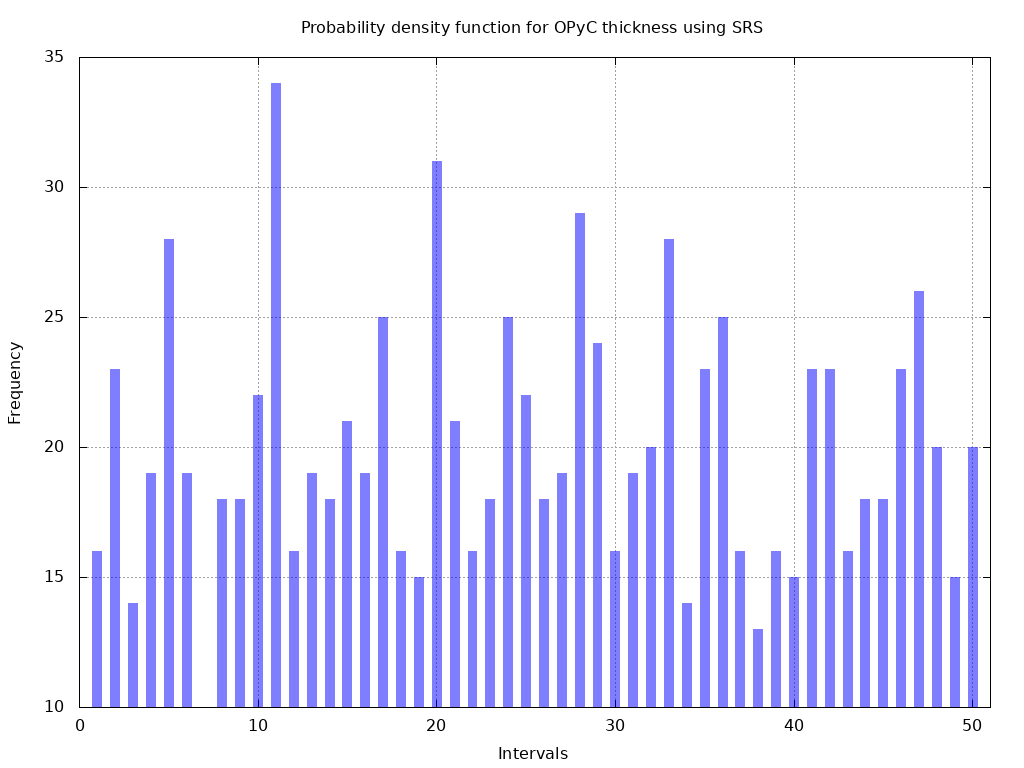
\includegraphics[width=130mm]{pics/SRS_Uniform_OPyC.png}}
\caption{Distribusi \textit{sample} yang diperoleh menggunakan distribusi \textit{uniform} serta metode (a). LHS dan (b). SRS}
\end{center}
\end{figure}

\begin{figure}[h!]
\begin{center}
\subfigure[]{\label{fig:triLHS}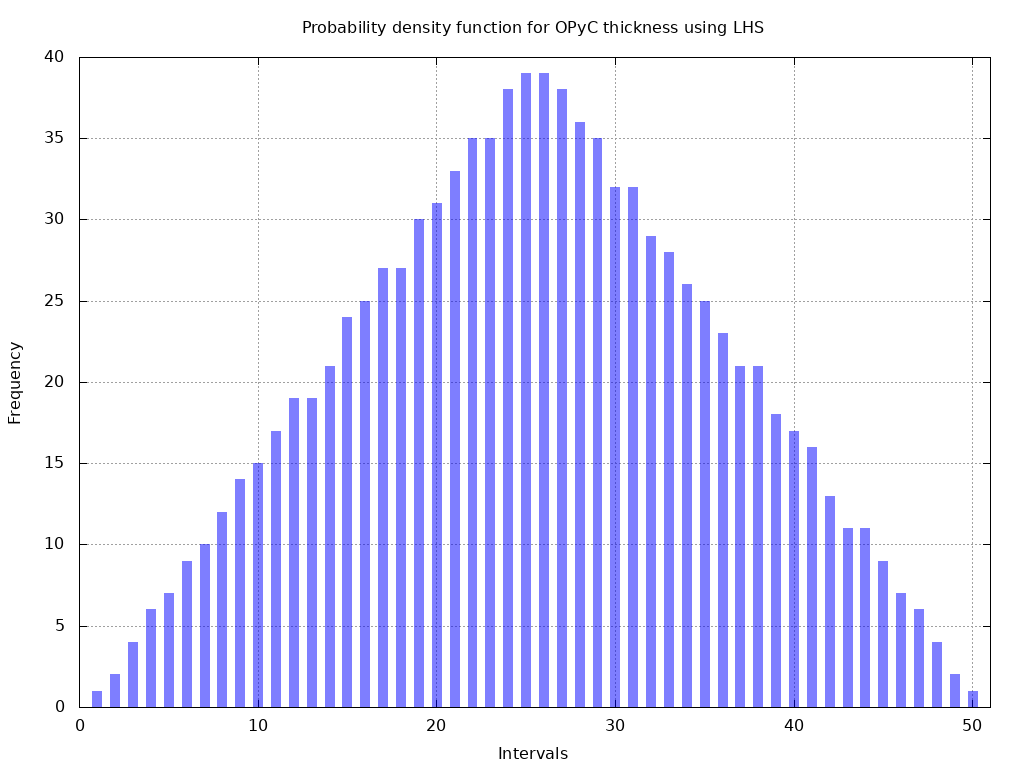
\includegraphics[width=130mm]{pics/LHS_Triangle_OPyC.png}}
\subfigure[]{\label{fig:triSRS}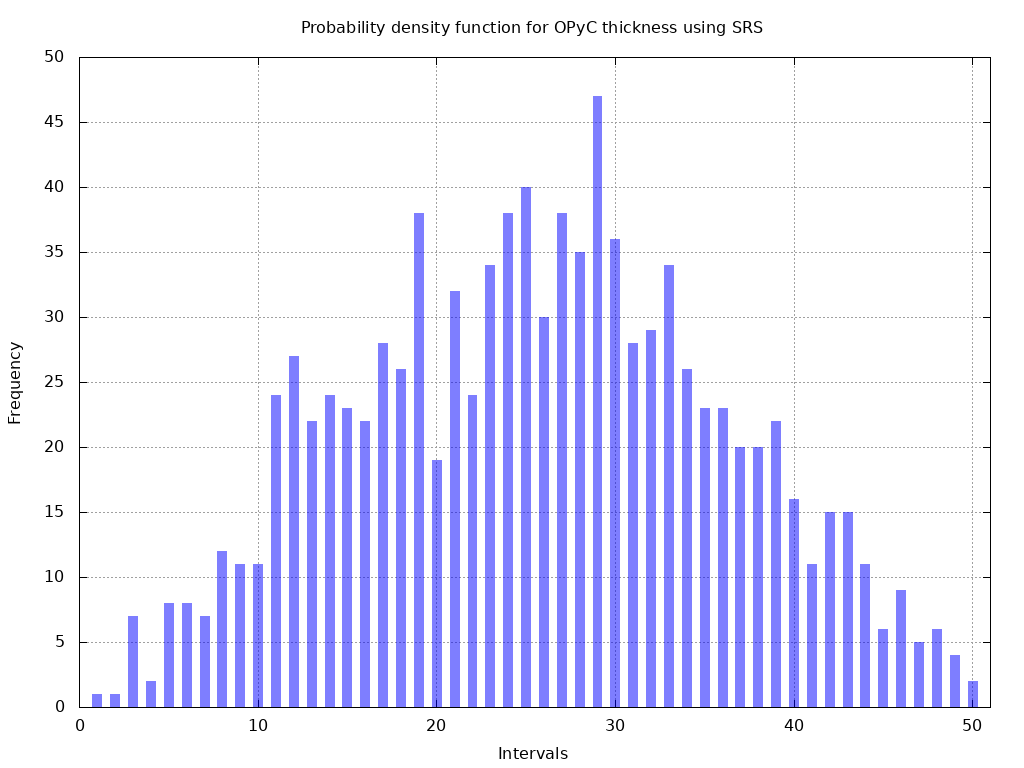
\includegraphics[width=130mm]{pics/SRS_Triangle_OPyC.png}}
\caption{Distribusi \textit{sample} yang diperoleh menggunakan distribusi triangular serta metode (a). LHS dan (b). SRS}
\end{center}
\end{figure}

Pengujian selanjutnya adalah untuk melihat dampak dari mempertimbangkan ketidakpastian pada setiap lapisan triso yang seragam dalam hal distribusi dan metode \textit{sampling}. Yang dimaksud dengan seragam tersebut adalah, jika skenario yang sedang dijalankan adalah menggunakan distribusi \textit{uniform} dengan metode sampling LHS, maka semua lapisan triso akan menggunakan distribusi dan metode \textit{sampling} yang sama. Kemudian, hasilnya akan disajikan dalam bentuk plot nilai rerata fraksi gagal dan penyimpangan bakunya ($\sigma$). Skenario ini seluruhnya dijalankan dengan menggunakan 100 \textit{sample}.

Gambar \ref{fig:stdUnifLHS} dan \ref{fig:stdUnifSRS} menunjukkan pola fraksi gagal yang diperoleh dari \textit{sample} yang diperoleh menggunakan distribusi \textit{uniform}, baik dengan metode LHS maupun SRS. Sedangkan Gambar \ref{fig:stdTriLHS} dan \ref{fig:stdTriSRS} adalah hasil dari pengujian serupa menggunakan \textit{sample} yang terdistribusi triangular.
\begin{figure}[h!]
\begin{center}
\subfigure[]{\label{fig:stdUnifLHS}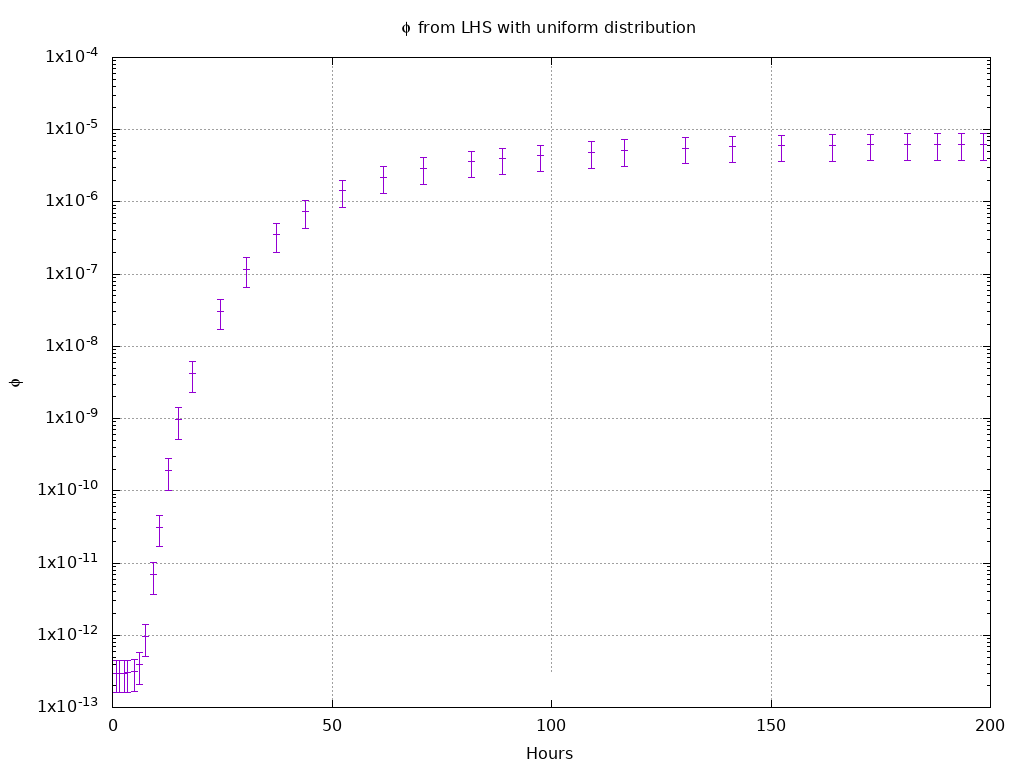
\includegraphics[width=130mm]{pics/stdDevUniformLHS.png}}
\subfigure[]{\label{fig:stdUnifSRS}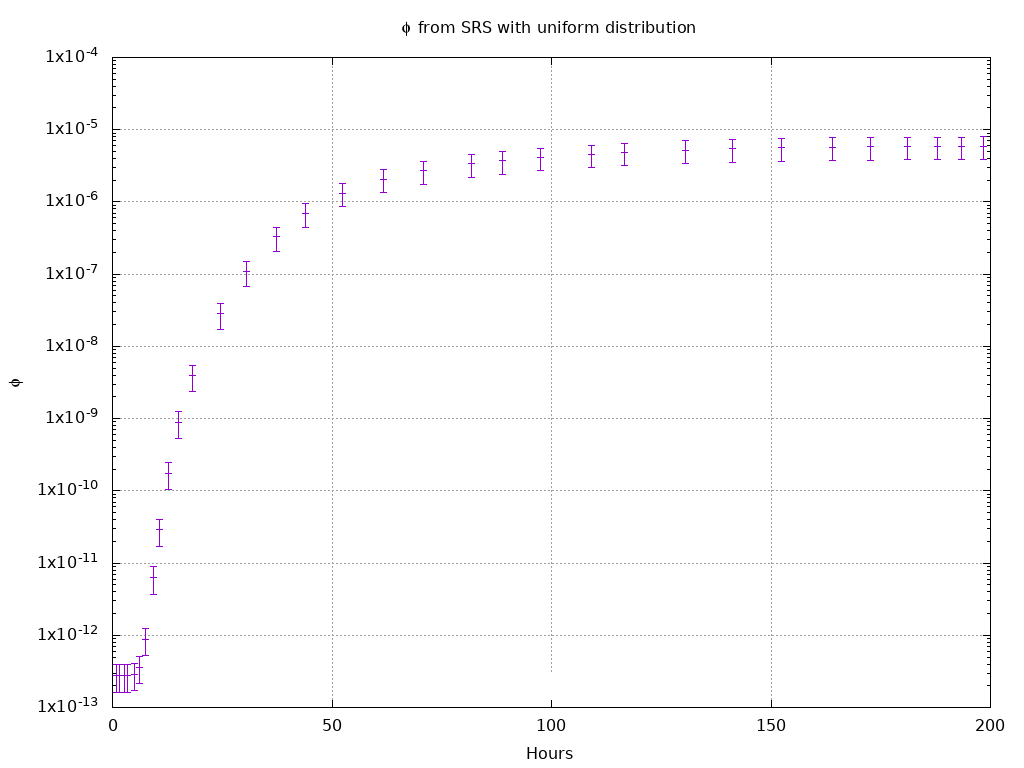
\includegraphics[width=130mm]{pics/stdDevUniformSRS.png}}
\caption{Nilai rerata dan $\sigma$ fraksi gagal partikel triso menggunakan metode $\sigma$  (a). LHS and (b). SRS dan distribusi \textit{uniform}}
\end{center}
\end{figure}

\begin{figure}[h!]
\begin{center}
\subfigure[]{\label{fig:stdTriLHS}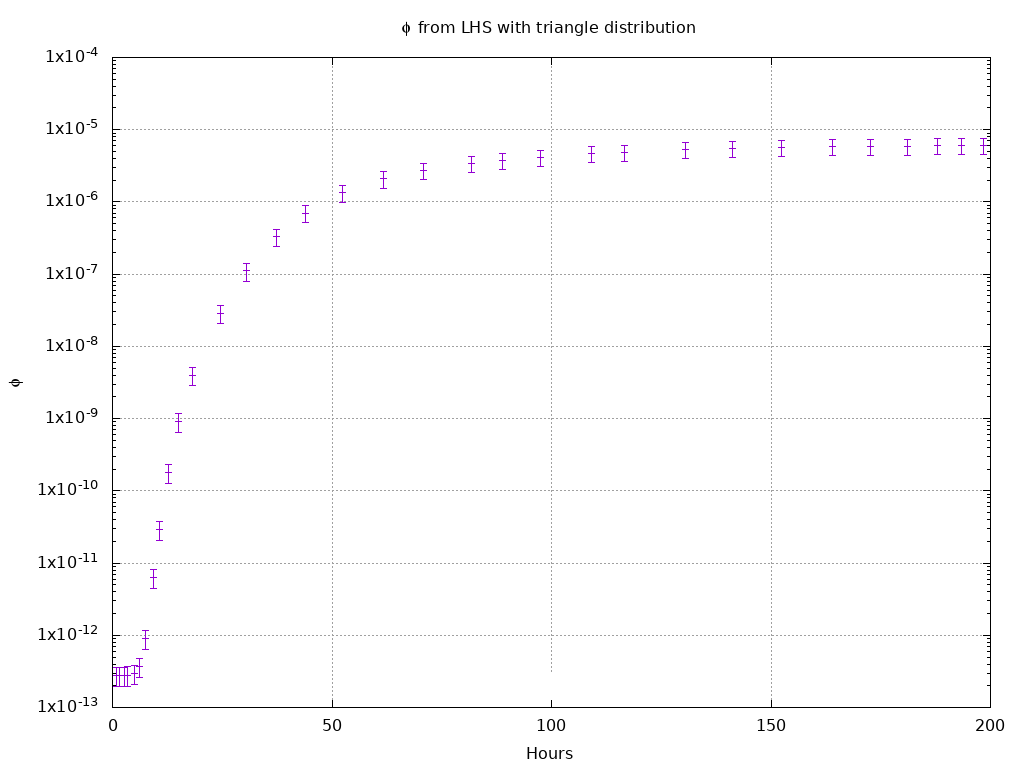
\includegraphics[width=130mm]{pics/stdDevTriangleLHS.png}}
\subfigure[]{\label{fig:stdTriSRS}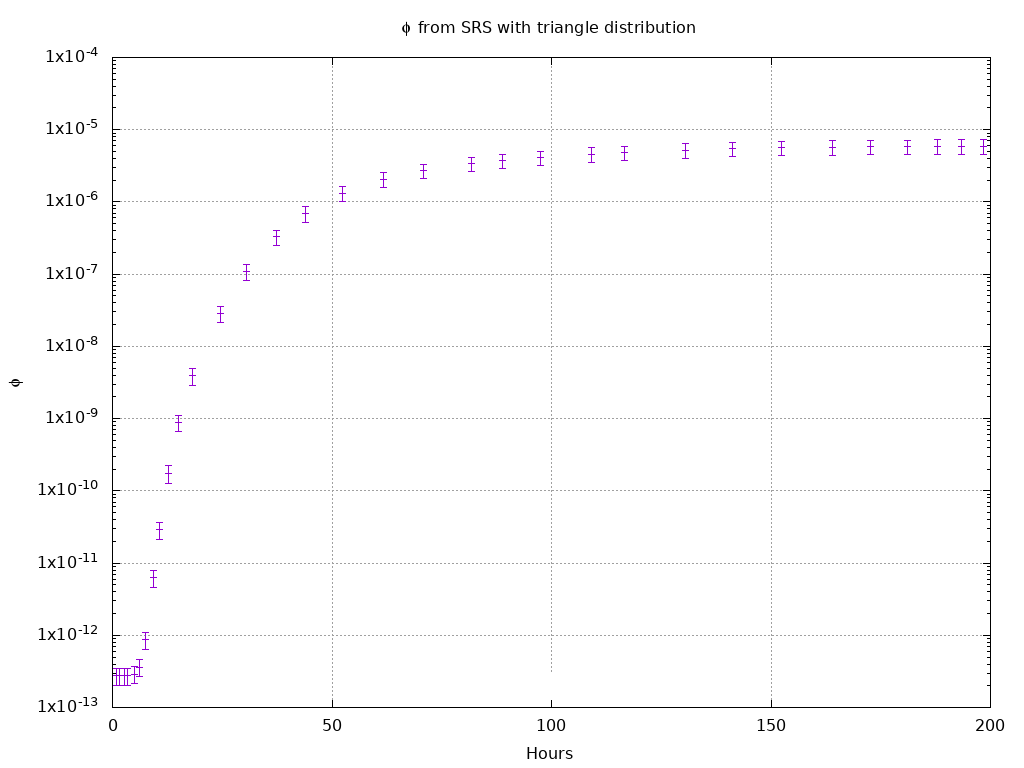
\includegraphics[width=130mm]{pics/stdDevTriangleSRS.png}}
\caption{Nilai rerata dan $\sigma$ fraksi gagal partikel triso menggunakan metode $\sigma$  (a). LHS and (b). SRS dan distribusi triangular}
\end{center}
\end{figure}

Dari perspektif distribusi \textit{sample}, diketahui bahwa distribusi \textit{uniform} menghasilkan $\sigma$ yang lebih besar daripada triangular. Hal ini dapat dipahami ketika kita melihat Gambar \ref{fig:triLHS} dan \ref{fig:triSRS}. Pada gambar dengan distribusi triangular tersebut, \textit{sample} yang berukuran tidak jauh dari nilai rerata adalah \textit{sample} dengan jumlah yang mayoritas. Secara statistik hal ini disebut sebagai kondisi di mana variasi \textit{sample} rendah. Hal ini berkebalikan dengan distribusi \textit{uniform} yang \textit{sample} yang terbentuk terdistribusi cukup seragam dalam rentang ketidakpastian.

Sedangkan dari perspektif metode sampling, LHS justru menghasilkan nilai $\sigma$ yang cenderung lebih besar daripada SRS. Hal ini dapat dipahami dari Gambar \ref{fig:unifLHS} dan \ref{fig:unifSRS}. Pada distribusi \textit{sample} yang diperoleh menggunakan SRS terdistribusi secara acak, sehingga ada rentang ketidakpastian yang tidak memiliki \textit{sample}. Kondisi seperti ini memungkinkan terjadinya efek saling menghilangkan variasi sehingga menghasilkan nilai $\sigma$ cenderung kecil.

Hasil terkahir memang belum valid karena fraksi gagal diperoleh dengan mensimulasi ketidakpastian secara bersamaan di setiap lapisan triso. Masih perlu dievaluasi pengaruh ketidakpastian di setiap lapisan secara terpisah terhadap fraksi gagal triso.

% Daftar Pustaka
\bibliographystyle{IEEEtran}
\bibliography{report}

\begin{appendix}
	%
% @author  Andreas Febrian
% @version 1.00 
% 
% Hanya sebuah pembatas bertuliskan LAMPIRAN ditengah halaman. 
% 

\begin{titlepage}
	\centering 
	\vspace*{6cm}
	\noindent \Huge{LAMPIRAN}
	\addChapter{LAMPIRAN}
\end{titlepage}

	\setcounter{page}{2}
	%-----------------------------------------------------------------------------%
\addChapter{Lampiran 1}
\chapter*{Lampiran 1: Contoh file input}
\label{lamp:inputExample}
%-----------------------------------------------------------------------------%
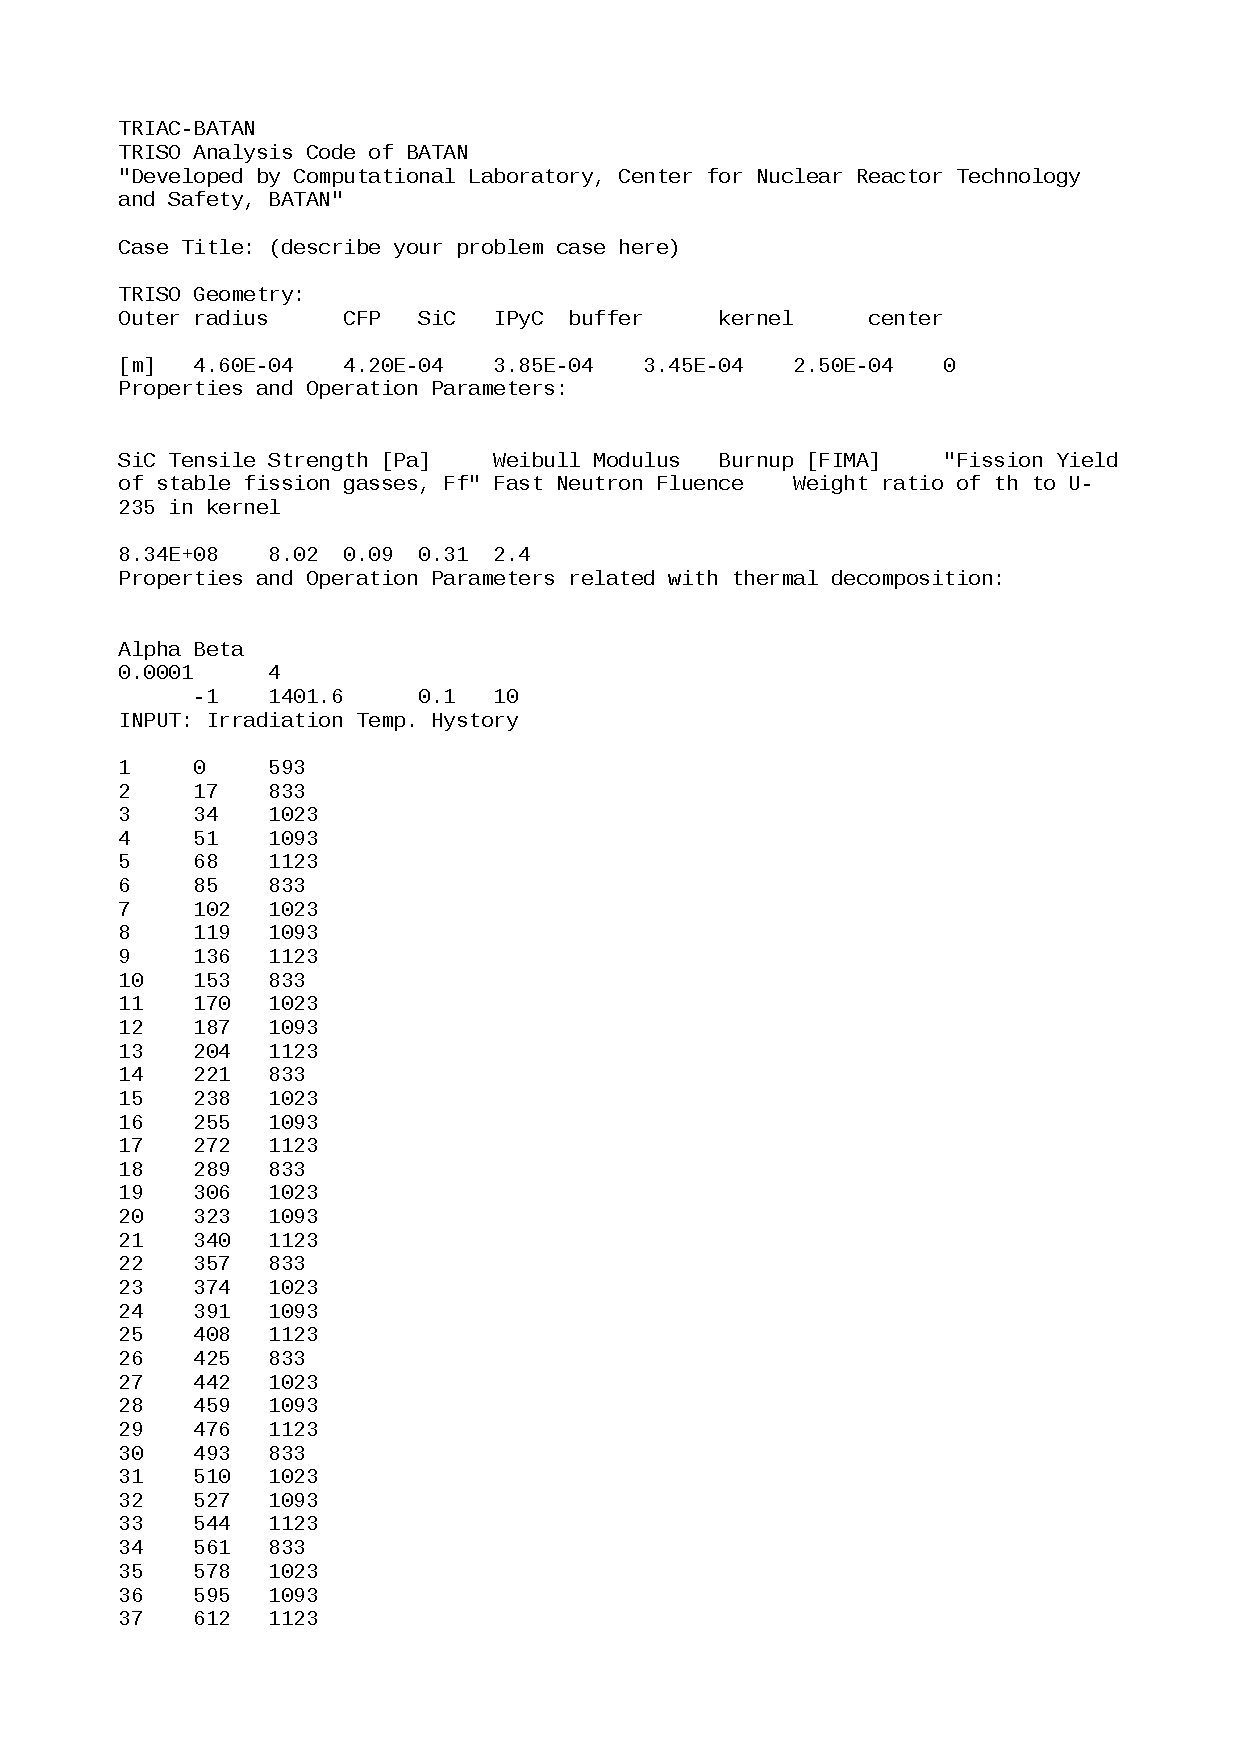
\includepdf[pages={1-}]{inputExample.pdf}
%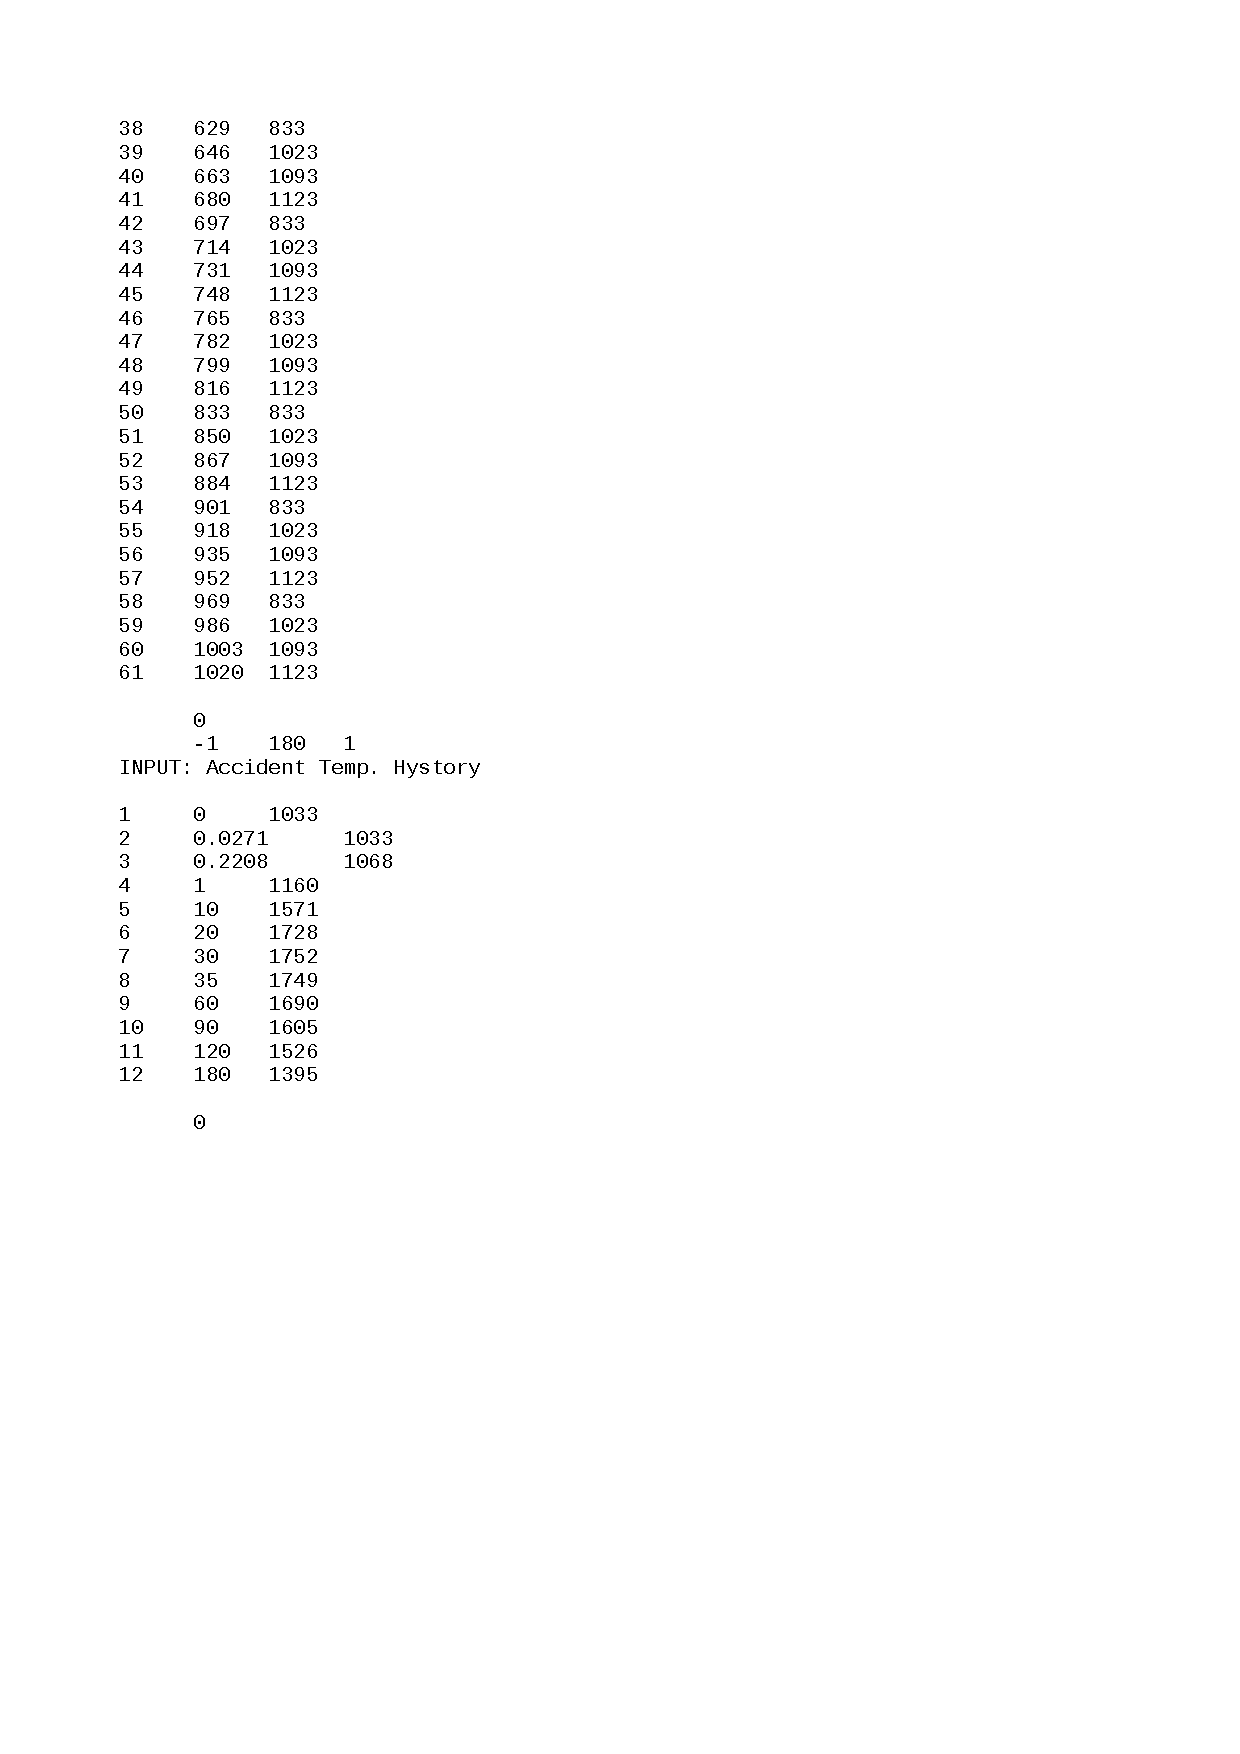
\includepdf{inputExample2}

\addChapter{Lampiran 2: InputData.py}
\chapter*{Lampiran 2: InputData.py}
\scriptsize
\lstinputlisting[language=python, numbers=left, numberstyle=\tiny, caption=InputData.py, showstringspaces=false, label=InputData.py]{../Uji/InputData.py}
\normalsize

\addChapter{Lampiran 3: interpolasi.py}
\chapter*{Lampiran 3: interpolasi.py}
\scriptsize
\lstinputlisting[language=python, numbers=left, numberstyle=\tiny, caption=Interpolasi.py, showstringspaces=false, label=Interpolasi.py]{../TRIAC/Interpolasi.py}
\normalsize

\addChapter{Lampiran 4: core.py}
\chapter*{Lampiran 4: core.py}
\scriptsize
\lstinputlisting[language=python, numbers=left, numberstyle=\tiny, caption=core.py, showstringspaces=false, label=core.py]{../Uji/core.py}
\normalsize

\addChapter{Lampiran 5: triac.py}
\chapter*{Lampiran 5: triac.py}
\scriptsize
\lstinputlisting[language=python, numbers=left, numberstyle=\tiny, caption=triac.py, showstringspaces=false, label=triac.py]{../Uji/triacc.py}
\normalsize

\end{appendix}

\end{document}
